\documentclass[lang=cn]{elegantbook}
\usepackage[utf8]{inputenc}
\usepackage{amssymb}
\usepackage{amsmath}
\usepackage{etoolbox}
\usepackage{xcolor}
\usepackage{enumerate}
\newcommand\wyc[1]{\bf\textcolor{cyan}{#1}}
\newcommand{\listsum}[3]{#1_0 #2^#3 + #1_1 #2^{#3 - 1} + \cdots + #1_{#3 - 1} #2 + #1_k}
\newcommand{\mean}[2]{\frac{#1_1 + #1_2 + \cdots + #1_#2}{#2}}
\newcommand{\mylim}[2]{\lim_{#1 \to \infty } #2}
\newcommand{\mylinelim}[2]{\lim\limits_{#1 \to \infty} #2}
\newcommand{\collect}[1]{\left\{ #1\right\}}
\newcommand{\funclim}[3]{\lim_{#1 \to #2 } #3}
\newcommand{\arccot}{\mathrm{arccot}}
\newcommand{\e}{\mathrm{e}}
\newcommand{\D}{\mathrm{d}}
\newcommand{\ch}{\mathrm{ch}}
\newcommand{\sh}{\mathrm{sh}}
% \th \eth is defined
\newcommand{\thx}{\mathrm{th}}
\newcommand{\cth}{\mathrm{cth}}

\newcommand{\der}[2]{\frac{\D #1}{\D #2}}
\newcommand{\dern}[3]{\frac{\D^#1 #2}{\D #3^#1}}

\graphicspath{{picture/}{figure/}}

\title{数学分析}
\author{hapo}
\date{\today}

\setcounter{tocdepth}{3}
\logo{nju-emblem.pdf}
\cover{cover.jpg}

\begin{document}

\maketitle
\frontmatter

\tableofcontents

\mainmatter
记录本书的原因是因为我觉得自己的数学分析实在太烂了。因此我决定使用费曼学习法。这是一个链式反应,在我学习随机过程的时候,我发现自己的概率论太差了,而当我学习概率论的时候,我又发现我的测度论太差了,而我学习测度论的时候,我最终发现,我差的是数学分析。而这个最初始的问题是我并没有系统地学过数学分析。而在学习数学分析的过程中,我发现我对好多概念并不明晰,这使得学习的进度缓慢,并且经常容易在概念上卡壳,而卡壳结束后又很快忘记。因此,为了能够更好地记住,我决定使用费曼学习法。在此,我记录下我学习数学分析的过程。

\chapter{集合与映射}
% 陈老视频1
\begin{definition}[集合]
{\bf 集合(集)}是具有某种特定性质的具体的或抽象的对象汇集的总体,其中的对象称为集合的元素。
\end{definition}
集合通常记为A, B, C, X, Y

元素通常记为s, t, a, b, x, y

x是集合S的元素, 记为$x\in S$
\chapter{实数的完备性}
\begin{introduction}
  \item 有理数的定义~\ref{def:rational-number}
  \item Bolzano-Weierstrass定理~\ref{theorem:Bolzano-Weierstrass}
  \item 数列极限的唯一性~\ref{theorem:limit-uniqueness}
  \item 数列极限的保序性逆命题~\ref{lemma:progression-order}

\end{introduction}
在本章中,我们将介绍实数的完备性。在介绍实数之前,我们需要将实数定义或者说引入。而对于实数的定义是有很多的,而我在此介绍无穷十进制小数表示和戴德金(Dedekind)分割。这部分我将结合陈纪修教授的教材和Ayumu的讲义。

在引入实数之前,我们需要先介绍有理数,而在介绍有理数之前,我们需要规定一些常用集合的记号。而介绍常用集合,则需要先介绍集合(set),在此我们并不介绍集合,我们暂时默认我们已经知道了集合的概念,将来我们会对该部分内容进行扩充。现在让我们来列举一些常用的集合。
\begin{definition}[常用集合表示]
$\mathbb{N} = \{ 1, 2, 3, \cdots, n, \cdots\}$

$\mathbb{Z} = \{ 0, \pm 1, \pm 2, \pm 3, \cdots, \pm n, \cdots \}$

$\mathbb{Z}^+ = \{ n | n \in \mathbb{Z}, n > 0 \}$
\end{definition}
在定义了以上的集合表示之后,我们就能以上的符号来表示有理数:
\begin{definition}[有理数] \label{def:rational-number} 
若一个数x可以表示成$\frac{q}{p}$的形式,其中$q \in \mathbb{Z}$, $p \in \mathbb{Z}^+$, 则称x为{\bf 有理数}(rational number)。而由有理数组成的集合称为{\bf 有理数集},有理数集常用$\mathbb{Q}$表示,其可以表示为:
\[ \mathbb{Q} = \{ x | x = \frac{q}{p}, q \in \mathbb{Z}, p \in \mathbb{Z}^+ \} \]
在这里, 我们可以看到p只需要属于$\mathbb{Z}^+$, 这是因为若x为负的, 我们总可以规定负号出现在分子上。
\end{definition}
有理数对加减乘除都封闭,并且我们在有理数上定义了大小关系,即有理数也是良序的。但是它并不能满足研究所需。例如,存在长度无法用有理数表示。并且有理数之间存在``空隙'',即有理数不连续。而在我们之后的研究中,我们往往需要研究连续性,因此我们需要对有理数进行扩充。在这之前,我们先来证明确实有一些数无法用有理数表示。


\begin{example}
$\sqrt{2}$不是有理数。
\end{example}
\begin{proof}
我们用反证法。假设$\sqrt{2}$为有理数, 那么存在$q \in \mathbb{Z}, p \in \mathbb{Z}^+$, $p, q$互质, 使得$\sqrt{2} = \frac{q}{p}$, 即$q^2 = 2p^2$。因为$q^2$可以被2整除, 即$q^2$为偶数, 则$q$为偶数。那么$q$可以表示为$q = 2m, m \in \mathbb{Z}$。代入上式中, 得$p^2 = 2m^2$, 即$p$也为偶数。这与互质矛盾, 因此假设不成立, $\sqrt{2}$不是有理数。
\end{proof}
\begin{example}
    若n不是完全平方数, 则$\sqrt{n}$不是有理数。
\end{example}
\begin{proof}
\end{proof}
除了以上举例的有些数无法用有理数表示以外, 有的函数在实数域和有理数域上的表现完全不一样,比如狄利克雷(dirichlet)函数:
\begin{equation*}
    D(x) = \left\{
        \begin{aligned}
            1 &\quad x\text{是有理数} \\
            0 &\quad x\text{是无理数}
        \end{aligned}
    \right.
\end{equation*}

% 陈老视频8
\begin{theorem}[确界存在定理---实数系连续性定理]
    非空有上界的数集必有上确界,非空有下界的数集必有下确界。
\end{theorem}
\begin{proof}
    
\end{proof}

% 陈老视频9
\section{数列极限}
\begin{definition}[数列极限的定义]
    对于数列$\{ a_n \}$, 存在一个实常数a, 对$\forall \epsilon > 0$, $\exists N \in \mathbb{Z}^+$,使得当$n > N$时,$|a_n-a| < \epsilon$成立,则称$\{ a_n \}${\bf 收敛}(convengent)于a或者$\{ a_n \}$的{\bf 极限}(limit)为a, 记作
    \[ \lim_{n \to \infty} a_n = a \text{\quad 或者 \quad}  a_n \to a(n \to +\infty)\]
    若不存在实数a, 满足上述性质, 则称数列$\{ a_n \}${\bf 发散}(divergent)。
\end{definition}
在这里定义邻域的概念:$a$的$\epsilon$邻域$O(a, \epsilon)$为:$(a-\epsilon, a+\epsilon)$。因此数列极限的定义也可以描述为: 当$n > N$时, $a_n$落在a的$\epsilon$邻域内。

并且,一个数列的极限还有以下的一些性质。首先, 一个数列是否收敛, 收敛的话, 收敛于哪个数, 这与数列的前有限项无关。这是因为, 假如数列收敛于A, 我对前K项做了修改, 那么$\forall \epsilon > 0$, 可以取$N' = \max\{K, N\}$, 此时$\left| x_n -A \right| < \epsilon$, 即极限依旧为A。又比如极限不存在时, 则$\exists \epsilon > 0$, $\forall N \in \mathbb{N}^+$, $\exists n > N$, $\left| x_n - A \right| > \epsilon$。此时, $\forall N > K$, $\exists n > N$, $\left| x_n -A \right| > \epsilon$, 那么$N < K$时也成立。因此在求极限的不等式时, 可以从选定的一个N开始,有时候会使得不等式的求解方便。

此外, $\epsilon$还可以限定为小于一定值, 在该限定下证明不等式成立。这是因为当$\epsilon \le c$时候, 存在了N, 使得$n > N$时成立, 那么当$\epsilon > c$时, 该N也能使得$n >N$时成立。

接下来我们定义一个特殊的数列极限: {\bf 无穷小量}。我们会在之后特殊讨论它, 例如无穷小量的阶。 
\begin{definition}[无穷小量的定义]
    以零为极限的变量称为{\bf 无穷小量}。
\end{definition}

\begin{example}
    证明:
    \[ \mylim{n}{\frac{n}{n+3}}= 1 \]
\end{example}
\begin{proof}
    令:
    \[ \left| \frac{n}{n+3} - 1 \right| = \frac{3}{n + 3} < \frac{3}{n} < \epsilon \]
    因此, 当$N = \left[ \frac{3}{\epsilon} \right] + 1$时, $\left| \frac{n}{n+3} - 1 \right| < \epsilon$
\end{proof}

\begin{example}
    证明:
    \[ \mylim{n}{q^n}= 0(0 < \left|q\right| < 1) \]
\end{example}
\begin{proof}
    因为$0< \left|q\right| < 1$, 则$\left|q^n\right| = \left|q\right|^n < \epsilon$, 则:
    \[ n > \frac{\lg(\epsilon)}{\lg(\left|q\right|)} \]
    因为$N \in \mathbb{N}^+$, 所以取$N = \max\left\{1, \left[ \frac{\lg(\epsilon)}{\lg(\left|q\right|)} \right]\right\}$, 当$n > N$时, $\left| q^n - 0 \right| < \epsilon$, 即:
    \[ \mylim{n}{q^n} = 0(0 < \left|q\right| < 1) \]
\end{proof}

% 陈老视频10
\begin{example}\label{example-chapter2-1}
    证明:
    \[ \lim_{n \to \infty } \sqrt[n]{a}= 1 (a > 1)\]
\end{example}
\begin{proof}
    因为$a > 1$, 所以$\left| \sqrt[n]{a} - 1 \right| =\sqrt[n]{a} - 1$:
    \begin{equation*}
        \sqrt[n]{a} - 1 = \sqrt[n]{1\cdot 1\cdot 1\cdots a} - 1 < \frac{(n - 1) + a}{n} - 1 < \frac{a - 1}{n} < \frac{a}{n} < \epsilon 
    \end{equation*}
    所以取$N = \left[ \frac{a}{\epsilon} \right] + 1$时, $\forall n > N$, $\left| \sqrt[n]{a} - 1\right| < \epsilon$, 即$\mylim{n}{\sqrt[n]{a}} = 1$。

    \framebox{陈老是这样证明的}:

    令$y_n = \sqrt[n]{a} - 1$, 则:
    \begin{equation*}
        a = (1 + y_n)^n = 1 + C_n^1 y_n + C_n^2 y_n^2 + \cdots + C_n^n y_n^n         
    \end{equation*}

    则:
    \[ 1 + ny_n < a \]
    即:
    \[ y_n < \frac{a - 1}{n} < \epsilon \]
    则取$N = \left[ \frac{a - 1}{\epsilon} \right] + 1$, , $\forall n > N$, $\left| \sqrt[n]{a} - 1\right| < \epsilon$, 即$\mylim{n}{\sqrt[n]{a}} = 1$
\end{proof}
\begin{remark}
    对于$\sqrt[n]{1+x}$利用均值不等式可以得到一个有意思的不等式:
    \begin{equation*}
        \sqrt[n]{1+x} < 1 + \frac{x}{n}
    \end{equation*}
\end{remark}
\begin{example}
    证明
    \[ \lim_{n \to \infty } \sqrt[n]{n}= 1 \]
\end{example}
\begin{proof}
    因为$n \ge 1$, 所以$\left| \sqrt[n]{n} - 1 \right| = \sqrt[n]{n} - 1$:
    \[ \sqrt[n]{n} -1 = \sqrt[n]{1\cdot 1\cdot 1\cdots \sqrt{n} \cdot \sqrt{n} } -1 < \frac{n-2+2\sqrt{n}}{n} - 1 < \frac{2}{\sqrt{n}} < \epsilon \]
    所以取$N = \left[ \frac{4}{\epsilon^2}\right] + 1$时, $\forall n > N$, $\left| \sqrt[n]{n} - 1\right| < \epsilon$, 即$\mylim{n}{\sqrt[n]{n}} = 1$。

    \framebox{陈老是这样证明的}:

    令$y_n = \sqrt[n]{n} - 1$, 则:
    \begin{equation*}
        n = (1 + y_n)^n = 1 + C_n^1 y_n + C_n^2 y_n^2 + \cdots + C_n^n y_n^n
    \end{equation*}
    则:
    \[ 1 + C_n^2 y_n^2 < n \]
    即
    \[ y_n < \sqrt{\frac{2}{n}} < \epsilon \]
    则取$N = \left[ \frac{2}{\epsilon^2} \right] + 1$, , $\forall n > N$, $\left| \sqrt[n]{n} - 1\right| < \epsilon$, 即$\mylim{n}{\sqrt[n]{n}} = 1$
\end{proof}

\begin{remark}
    实际上, 用以上两种方法, 我们可以证明$\mylim{n}{\sqrt[n]{n^k}} = 1, (k \in \mathbb{N}^+)$。
\end{remark}

\begin{example}
    证明:
    \[ \lim_{n \to \infty } \sqrt[n]{n^k}= 1, (k \in \mathbb{N}^+) \]
\end{example}
\begin{proof}
    因为$n \ge 1$, 所以$\left| \sqrt[n]{n^k} - 1 \right| = \sqrt[n]{n^k} - 1$:
    \[ \sqrt[n]{n} -1 = \sqrt[n]{1\cdot 1\cdot 1\cdots \sqrt{n} \cdot \sqrt{n} \cdot \sqrt{n} } -1 < \frac{n-2k+2k\sqrt{n}}{n} - 1 < \frac{2k}{\sqrt{n}} < \epsilon \]
    所以取$N = \left[ \frac{4k^2}{\epsilon^2}\right] + 1$时, $\forall n > N$, $\left| \sqrt[n]{n^k} - 1\right| < \epsilon$, 即$\mylim{n}{\sqrt[n]{n^k}} = 1$。

    \framebox{陈老证明方法}:
    取$n > 2k$, 令$y_n = \sqrt[n]{n^k} - 1$, 则:
    \begin{equation*}
        n^k = (1 + y_n)^n = 1 + C_n^1 y_n + \cdot + C_n^{k+1}y_n^{k+1} + \cdots + C_n^n y_n^n
    \end{equation*}
    则:
    \begin{equation*}
        \frac{(n-k)^{k+1}}{{(k+1)}^{k+1}}y_n^{k+1} < C_n^{k+1}y_n^{k+1} < n^k
    \end{equation*}
    则:
    \begin{equation*}
        y_n < (k+1)\sqrt[k+1]{\frac{n^k}{(n-k)^n(n-k)}}
    \end{equation*}
    因为$n > 2k$, 则$n-k = \frac{n}{2} + \frac{n}{2} - k > \frac{n}{2}$, 所以:
    \begin{equation*}
        yn < (k+1)\sqrt[k+1]{\frac{n^k}{(n-k)^n(n-k)}} < (k+1)\sqrt[k+1]{\frac{2^k}{(n-k)}} < \epsilon
    \end{equation*}
    则取:
    \begin{equation*}
        N = \max\left\{ 2k, \left[ \frac{2^k}{\left( \frac{\epsilon}{k+1} \right)^{k+1}}\right] + k + 1\right\}
    \end{equation*}
    当$n > N$时,$yn < \epsilon$, 即$\mylim{n}{\sqrt[n]{n^k}} = 1$
\end{proof}
\begin{remark}
    在知道极限的四则运算法则后, $\sqrt[n]{n^k} = \left(\sqrt[n]{n}\right)^k$可以很快得出极限为1。
\end{remark}


\begin{example}\label{example-chapter2-2}
    设$a_n > 0$,$\lim_{n \to \infty} a_n = a$,证明
    \begin{equation*}
        \mylim{n}{\mean{a}{n}} = a
    \end{equation*}
\end{example}
\begin{proof}
    \def\tmp#1{\left| a_{#1} - a \right|}
    \edef\tmpmax#1{\max\left\{#1\right\}}
    因为$\mylim{n}{a_n} = a$, 所以$\exists N \in \mathbb{N}^+$, $\forall n > N$, $\tmp{n} < \frac{\epsilon}{2}$。
    \begin{equation*}
        \begin{aligned}
            \left| \mean{a}{n} -a \right| &\le  \frac{\tmp{1} + \tmp{2} + \cdots + \tmp{n}}{n} \\
            & = \frac{\tmp{1} + \cdots + \tmp{N}}{n} + \frac{\tmp{N+1} + \cdots + \tmp{n}}{n} 
        \end{aligned}    
    \end{equation*}
    对于后一项, 当$n > N$时, 有:
    \begin{equation*}
        \frac{\tmp{N+1} + \cdots + \tmp{n}}{n} < \frac{n\epsilon/2}{n} < \frac{\epsilon}{2}
    \end{equation*}
    对于前一项, 因为N为一个有限数, 则取$M = \tmpmax{\tmp{1}, \tmp{2}, \cdots, \tmp{N}}$, 因此:
    \begin{equation*}
        \frac{\tmp{1} + \cdots + \tmp{N}}{n} < \frac{NM}{n}
    \end{equation*}
    因此取$N_1 = \left[ \frac{2NM}{\epsilon} + 1 \right]$, 当$n > N_1$时:
    \begin{equation*}
        \frac{\tmp{1} + \cdots + \tmp{N}}{n} < \frac{\epsilon}{2}
    \end{equation*}
    因此, 取$N_2 = \tmpmax{N, N_1}$, 当$n > N_2$时:
    \begin{equation*}
        \mean{a}{n} < \epsilon
    \end{equation*}
    即:
    \begin{equation*}
        \mylim{n}{\mean{a}{n}} = a
    \end{equation*}
\end{proof}

在给出数列极限的定义之后, 我们来考察下数列极限的性质。因为现在我们只讲了定义, 如果求所有的导数都从定义出发, 那么过程会极其地繁琐。因此我们需要总结规律, 使得我们能够方便地求解数列极限。
\begin{theorem}[数列极限的唯一性]\label{theorem:limit-uniqueness}
    若
    \begin{equation*}
        \mylim{n}{x_n} = a, \mylim{n}{x_n} = b
    \end{equation*}
    则
    \begin{equation*}
        a = b
    \end{equation*}
\end{theorem}
\begin{remark}
    以下我不再写$N \in \mathbb{N}^+$, 因为过于冗余。
\end{remark}
\begin{proof}
    \framebox{证法一(陈老版本)}: $\forall \epsilon > 0$, $\exists N_1$, $\forall n > N_1$, $\left| a_n - a \right|< \frac{\epsilon}{2}$。$\exists N_2$, $\forall n > N_2$, $\left| b_n - b \right|< \frac{\epsilon}{2}$。所以$\forall n > \max\{N_1, N_2\}$, 有:
    \begin{equation*}
        \left| a - b \right| = \left| (a - a_n) - (b - a_n) \right| \le \left| a_n - a \right| + \left| a_n - b \right| < \frac{\epsilon}{2} + \frac{\epsilon}{2} = \epsilon
    \end{equation*}
    即$\forall \epsilon$, $\forall n > \max\{N_1, N_2\}$, $\left| a - b \right| < \epsilon$。$\left| a - b \right| < \epsilon$要对所有的$\epsilon$和$n$都成立, 因此$\left| a - b \right| = 0$, 即$a = b$。若$a \neq b$, 则可取$\epsilon = \frac{\left| a - b \right|}{2}$, 使得$\exists n$使不等式不成立。

    \begin{remark}
        也可以把$\{a\}$看作一个恒等序列, 则$\forall \epsilon > 0$, $\exists N$, $\forall n > N$, $\left| a - b \right| < \epsilon$, 即恒等数列$\{a\}$的极限为b, 则$a = b$。
    \end{remark}

    \framebox{证法二}:用反证法, 设$a > b$, 取$\epsilon = \frac{a - b}{2}$, 则$\exists N_1$, $\forall n > N_1$, $\left| a_n - a \right| < \frac{a - b}{2}$, 则$a_n > \frac{a + b}{2}$。同理可得: $\exists N_2$, $\forall n > N_2$, $a_n < \frac{a + b}{2}$。则$\forall n > \max\{N_1, N_2\}$, $\frac{a+b}{2} < a_n < \frac{a+b}{2}$, 存在矛盾, 即$a \le b$。同理可以证$a \ge b$, 因此$a = b$。
\end{proof}
\begin{remark}
    唯一性表明了收敛的数列极限$a$有且只有一个, 在定义中只说了$\exists a$, 并没有限定$a$的个数, 唯一性使得当我们求得一个极限时, 不用再去找别的极限值。
\end{remark}

接下来我们再来看数列的有界性, 有界性也是极限非常重要的性质, 很多时候可以帮助我们放大不等式。

\begin{definition}\label{definition:limit-bound}
    \begin{enumerate}
        \item 对于数列$\collect{x_n}$, 若$\exists M \in \mathbb{R}$, $\forall n \in \mathbb{N}^+$, 成立$x_n \le M$, 则称M是$\collect{x_n}$的一个上界, 或称$\collect{x_n}$有上界。
        \item 对于数列$\collect{x_n}$, 若$\exists m \in \mathbb{R}$, $\forall n \in \mathbb{N}^+$, 成立$x_n \ge m$, 则称m是$\collect{x_n}$的一个下界, 或称$\collect{x_n}$有下界。
    \end{enumerate}
    $\collect{x_n}$既有上界又有下界, 则称$\collect{x_n}$有界。

    $\collect{x_n}$有界的另一个定义:$\exists X \in \mathbb{R}^+$, $\forall n \in \mathbb{N}^+$, 成立$\left| x_n \right| \le X$。
\end{definition}
\begin{remark}
    我们先说明下这两个定义等价: 若$\collect{x_n}$有上界有下界, 则$\forall n \in \mathbb{N}^+$, $m \le x_n \le M$, 则$\left| x_n \right| \le \max\left\{ |m|, |M|\right\}$, 则我们找到了$X = \max\left\{ |m|, |M|\right\}$。若$\collect{x_n}$有界,即$\exists X \in \mathbb{R}^+$, $\forall n \in \mathbb{N}^+$, $\left| x_n \right| \le X$, 则$\forall n \in \mathbb{N}^+$, $-X \le x_n \le X$, 则我们找到了$m = -X, M = X$。
\end{remark}

\begin{theorem}[数列极限的有界性]\label{theorem:limit-bound}
    若$\{ x_n \}$的极限存在,则$\{ x_n \}$有界。
\end{theorem}
\begin{proof}
    设$\collect{x_n}$的极限为$a$, 取$\epsilon = 1$, 则$\exists N$, $\forall n > N$, $\left| x_n - a \right| < 1$, 则$a - 1 < x_n < a + 1$。

    因为$N$是一个固定数, 则取$m = \min\{x_1, x_2, \cdots, x_N, a - 1\}$, $M = \max\{x_1, x_2, \cdots, x_N, a + 1\}$, $\forall n \in \mathbb{N}^+$, $m \le x_n \le M$。
\end{proof}
% 陈老视频11
\begin{theorem}[数列极限的保序性]\label{theorem:progression-order}
    存在两个数列$\{ x_n \}$和$\{ y_n \}$,并且
    \[ \mylim{n}{x_n} = a, \mylim{n}{y_n} = b, \text{\quad 且 \quad}a < b \]则$\exists N \in \mathbb{Z}^+$,当$n > N$时,$x_n < y_n$。
\end{theorem}
\begin{proof}
    取$\epsilon = \frac{b-a}{2}$, 则$\exists N_1$, $\forall a > N_1$, $\left| x_n - a \right| < \frac{b-a}{2}$, 即:
    \begin{equation*}
        x_n -a < \frac{b-a}{2} \rightarrow x_n < \frac{b+a}{2}
    \end{equation*}
    同理, $\exists N_2$, $\forall n > N_2$, $\left| y_n - b \right| < \frac{b-a}{2}$, 即:
    \begin{equation*}
        y_n - b > -\frac{b-a}{2} \rightarrow y_n > \frac{a+b}{2}
    \end{equation*}
    即$\forall n > \max\{N_1, N_2\}$, $x_n < \frac{a+b}{2} < y_n$。

    \qed
\end{proof}

\begin{lemma}[数列极限的保序性逆命题]\label{lemma:progression-order}
    对于$\mylim{n}{x_n} = a,\mylim{n}{x_n} = b$, 若$\exists N \in \mathbb{N}^+$, $\forall n > N$, $x_n \le y_n$, 则$a \le b$。 
\end{lemma}
\begin{proof}
    \framebox{反证法}: 若$a > b$, 则$\exists N_1$, $\forall n > N_1$, $x_n > y_n$, 则$\forall, n > \max\{N, N_1\}$, $x_n > y_n$, 这与$\forall n > N$, $x_n \le y_n$条件矛盾, 则假设不成立。

    \qed
\end{proof}
\begin{remark}
    \begin{enumerate}
        \item $\exists N$, $forall n > N$, $x_n < y_n$, 并不能推出$a < b$, 例如$\collect{x_n = \frac{1}{2n}}$和$\collect{y_n = \frac{1}{n}}$, 它们的极限都是0。
        \item 可以直接从极限存在的情况下的逆否命题的角度思考该命题。写出定理~\ref{theorem:progression-order}的逆否命题: 对于$\mylim{n}{x_n} = a,\mylim{n}{x_n} = b$, $\forall N$, $\exists n > N$, $x_n \ge y_n$, 则$a \ge b$, $\exists N$, $\forall n > N$, $x_n \ge y_n$满足该情况, 因此$a \ge b$。
    \end{enumerate}
\end{remark}

\begin{lemma}
    \begin{enumerate}
        \item 若$\mylim{n}{y_n} = b > 0$, 则$\exists N \in \mathbb{N}^+$, $\forall n > N$, $y_n > \frac{b}{2} > 0 $。
        \item 若$\mylim{n}{y_n} = b < 0$, 则$\exists N \in \mathbb{N}^+$, $\forall n > N$, $y_n < \frac{b}{2} < 0 $。
    \end{enumerate}
\end{lemma}
\begin{proof}
    利用数列极限的保序性证明。当$b > 0$时,取$\collect{x_n = \frac{b}{2}}$, 则$\mylim{n}{x_n} = \frac{b}{2} < b$, 由数列极限的保序性可知,$\exists N \in \mathbb{N}^+$, $\forall n > N$, 有$y_n > x_n = \frac{b}{2}$。 
    
    \qed

    同理可证明$b < 0$的情况。
\end{proof}
以上推论可以合起来写为:
\begin{lemma}\label{lemma:progression-order-b}
    若$\mylim{n}{y_n} = b \neq 0$, 则$\exists N \in \mathbb{N}^+$, $\forall n > N$, $\left| y_n \right|> \frac{\left| b \right|}{2} > 0 $。
\end{lemma}
\begin{proof}
    除了上一个推论那样分开来证明, 还可以如下证明:
    $\mylim{n}{y_n} = b$, 即$\forall \epsilon > 0$, $\exists N \in \mathbb{N}^+$, $\forall n > N$, $\left| y_n - b\right| < \epsilon$。

    由三角不等式得:
    \begin{equation*}
        \left| y_n - b\right| \ge \left| \left| y_n \right| - \left| b \right| \right|
    \end{equation*}
    即:
    \begin{equation*}
        \left| \left| y_n \right| - \left| b \right| \right| \le \left| y_n - b\right| < \epsilon
    \end{equation*}
    因此$\mylim{n}{\left| y_n \right|} = \left| b \right|$。之后的证明同上。
\end{proof}

\begin{theorem}[数列极限的夹逼性定理]
    对于数列$\collect{x_n}$, $\collect{y_n}$, $\collect{z_n}$, 若$\exists N \in \mathbb{N}^+$, $\forall n > N$, 成立$x_n \le y_n \le z_n$, 且$\mylim{n}{x_n} = \mylim{n}{z_n} = a$, 则$\mylim{n}{y_n} = a$
\end{theorem}
\begin{proof}
    $\forall \epsilon$, $\exists N_1 \in \mathbb{N}^+$, $\forall n > N_1$, $\left| x_n - a\right| < \epsilon$, 即$x_n -a > -\epsilon$。

    同理, $\forall \epsilon$, $\exists N_2 \in \mathbb{N}^+$, $\forall n > N_2$, $\left| y_n - a\right| < \epsilon$, 即$z_n -a < \epsilon$。

    取$N = \max\left\{ N_1, N_2 \right\}$, 则:
    \begin{equation*}
        -\epsilon < x_n - a < y_n - a < z_n - a < \epsilon
    \end{equation*}
    即: 
    \begin{equation*}
        -\epsilon < y_n - a <\epsilon
    \end{equation*}
    即:
    \begin{equation*}
        \left| y_n - a \right| < \epsilon
    \end{equation*}
    总结起来即为:
    $\forall \epsilon$, $\exists N \in \mathbb{N}^+$, $\forall n > N$, $\left| y_n - a\right| < \epsilon$, 即$\mylim{n}{y_n} = a$。

    \qed
\end{proof}
\begin{example}
    求: 
    \begin{equation*}
        \mylim{n}{\left(\sqrt{n+1} - \sqrt{n}\right)}
    \end{equation*}
\end{example}
\begin{proof}
    因为$\sqrt{n+1} > \sqrt{n}$, 所以$\sqrt{n+1} - \sqrt{n} > 0$。

    又因为:
    \begin{equation*}
        \sqrt{n+1}-\sqrt{n} = \frac{1}{\sqrt{n+1}+\sqrt{n}} < \frac{1}{2\sqrt{n}}
    \end{equation*}
    因此:
    \begin{equation*}
        0 < \sqrt{n+1} - \sqrt{n} < \frac{1}{2\sqrt{n}}
    \end{equation*}
    又因为$\mylim{n}{\frac{1}{2\sqrt{n}}} = 0$, 所以根据夹逼定理:
    \begin{equation*}
        \mylim{n}{\left(\sqrt{n+1}-\sqrt{n}\right)} = 0
    \end{equation*}
\end{proof}
\begin{example}
    证明:
    \begin{equation*}
        \mylim{n}{\left( a_1^n + a_2^n + \cdots + a_p^n \right)^\frac{1}{n}} = \max_{1 \le i \le p}\{a_i\}
    \end{equation*}
    其中$a_1, a_2, \cdots, a_p > 0$, 且为常数。
\end{example}
\begin{proof}
    \def\tmp{\left(a_1^n + a_2^n + \cdots + a_p^n\right)^{\frac{1}{n}}}
    设$M = \max_{1 \le i \le p}\{a_i\}$, 则
    \begin{equation*}
        \begin{aligned}
            \tmp > M \\
            \tmp \le p^{\frac{1}{n}}M 
        \end{aligned}
    \end{equation*}
    在之前的证明中我们已经证明$\mylim{n}{\sqrt[n]{p}} = 1$, 因此根据夹逼定理:
    \begin{equation*}
        \mylim{n}{\tmp} = M
    \end{equation*}

    \qed
\end{proof}

\begin{example}
    用夹逼定理证明:
    \begin{equation*}
        \mylim{n}{\sqrt[n]{n}} = 1
    \end{equation*}
\end{example}
\begin{proof}
    这个用夹逼定理的证明实际上和之前提到的方法1接近, 即利用
    \begin{equation*}
        \sqrt[n]{n} = \sqrt[n]{1\cdot1\cdot1\cdots\sqrt{n}\cdot\sqrt{n}} <\frac{n-2+2\sqrt{n}}{n} < \frac{2}{\sqrt{n}} + 1
    \end{equation*}
\end{proof}

\begin{example}
    用夹逼定理证明:
    \begin{equation*}
        \mylim{n}{\sqrt[n]{n^2}} = 1
    \end{equation*}
\end{example}
\begin{proof}
    这个用夹逼定理的证明实际上也和之前提到的方法1接近, 即利用
    \begin{equation*}
        \sqrt[n]{n^2} = \sqrt[n]{1\cdot1\cdot1\cdots\sqrt{n}\cdot\sqrt{n}\cdot\sqrt{n}\cdot\sqrt{n}} <\frac{n-4+4\sqrt{n}}{n} < \frac{4}{\sqrt{n}} + 1
    \end{equation*}
\end{proof}
% 陈老视频12
下面再来介绍下数列极限的四则运算, 有了四则运算法则我们可以快速地计算极限。推导四则运算法则需要用到数列极限的有界性。
\begin{theorem}[数列极限的四则运算]
    若$\lim\limits_{n \to \infty} x_n = a$, $\lim\limits_{n \to \infty} y_n = b$,则
    \begin{enumerate}
        \item $\mylim{n}{(\alpha x_n + \beta y_n)} = \alpha a + \beta b$
        \item $\mylim{n}{(x_n y_n)} = ab$
        \item $\mylim{n}{(\frac{x_n}{y_n})} = \frac{a}{b}(b \neq 0)$
    \end{enumerate}
\end{theorem}
\begin{proof}
    首先根据收敛数列的有界性有: $\exists X > 0$, $\left| y_n \right| \le X$。

    \begin{enumerate}
        \item 证明: $\mylim{n}{(\alpha x_n + \beta y_n)} = \alpha a + \beta$ b。
        
        $\forall \epsilon$, $\exists N_1$, $\forall n > N_1$, $\left| x_n - a \right| < \frac{\epsilon}{|\alpha|+|\beta|}$; $\forall \epsilon$, $\exists N_2$, $\forall n > N_2$, $\left| y_n - b \right| < \frac{\epsilon}{|\alpha|+|\beta|}$。

        则$\forall \epsilon$, $\exists N = \max\{N_1, N_2\}$, $forall n > N$, 有:
        \begin{equation*}
            \left| \alpha x_n + \beta y_n - \alpha a - \beta b\right| \le |\alpha||x_n-a| + |\beta||y_n-b| < \epsilon
        \end{equation*}
        即:
        \begin{equation*}
            \mylim{n}{(\alpha x_n + \beta y_n)} = \alpha a + \beta b
        \end{equation*}
        \qed
        \item 证明: $\mylim{n}{(x_n y_n)} = ab$
        
        \begin{equation*}
            | x_ny_n - ab | = |x_ny_n - ay_n +ay_n - ab| \le | x_n - a||y_n| + |a||y_n - b| \le X|x_n-a| +|a||y_n-b| 
        \end{equation*}
        $\forall \epsilon$, $\exists N_1, N_2$, $\forall n > N_1$, $|x_n - a| < \frac{\epsilon}{X+|a|}$, $\forall n > N_2$, $|y_n - b| < \frac{\epsilon}{X+|a|}$。则$\forall n > \max\{N_1, N_2\}$, 有
        \begin{equation*}
            | x_ny_n - ab | < \epsilon
        \end{equation*}
        即:
        \begin{equation*}
            \mylim{n}{(x_n y_n)} = ab
        \end{equation*}
        \qed
        \item 证明: $\mylim{n}{(\frac{x_n}{y_n})} = \frac{a}{b}(b \neq 0)$
        
        因为$\mylim{n}{y_n} = b \neq 0$, 根据引理~\ref{lemma:progression-order-b}: $\exists N_0$, $\forall n > N_0$, $|y_n| > \frac{|b|}{2} > 0$。则:
        \begin{equation*}
            \left|\frac{x_n}{y_n} - \frac{a}{b} \right| = \frac{|bx_n - ay_n|}{|b||y_n|} < \frac{2|bx_n-ab+ab-ay_n|}{|b|^2} \le \frac{2(|b||x_n-a|+|a||y_n-b|)}{|b|^2}
        \end{equation*}
        $\forall \epsilon$, $\exists N_1, N_2$, $\forall n > N_1$, $|x_n - a| < \frac{|b|^2\epsilon}{2(|a|+|b|)}$, $\forall n > N_2$, $|y_n - b| < \frac{|b|^2\epsilon}{2(|a|+|b|)}$。则$\forall n > \max\{N_0, N_1, N_2\}$:
        \begin{equation*}
            \left| \frac{x_n}{y_n} - \frac{a}{b} \right| < \epsilon
        \end{equation*}
        即:
        \begin{equation*}
            \mylim{n}{(\frac{x_n}{y_n})} = \frac{a}{b}
        \end{equation*}
        \qed
    \end{enumerate}
\end{proof}
\begin{remark}
    \begin{enumerate}
        \item 对于第三个式子, 我们还可以先证明$\mylim{n}{\frac{1}{y_n}} = \frac{1}{b}$, 再用第二个式子, 这样的方式简化运算。
        \item 四则运算的适用范围是极限存在, 发散的情况下则不适用了。
    \end{enumerate}
\end{remark}

\begin{example}
    求:
    \begin{equation*}
        \mylim{n}{\frac{5^{n+1}-(-2)^n}{3 \cdot 5^n + 2\cdot 3^n}} 
    \end{equation*}
\end{example}
\begin{proof}
    上下同除以$5^n$, 则:
    \begin{equation*}
        \frac{5^{n+1}-(-2)^n}{3 \cdot 5^n + 2\cdot 3^n} = \frac{5-\left(-\frac{2}{5}\right)^n}{3+2\left(\frac{3}{5}\right)^n}
    \end{equation*}
    根据极限的四则运算得:
    \begin{equation*}
        \mylim{n}{\frac{5^{n+1}-(-2)^n}{3 \cdot 5^n + 2\cdot 3^n}} = \frac{5}{3}
    \end{equation*}
\end{proof}

\begin{example}
    当$a > 0$时, 证明:
    \begin{equation*}
        \mylim{n}{\sqrt[n]{a}} = 1
    \end{equation*}
\end{example}
\begin{proof}
    在例题~\ref{example-chapter2-1}中我们已经证明了当$a > 1$时:
    \begin{equation*}
        \mylim{n}{\sqrt[n]{a}} = 1
    \end{equation*}
    当$a = 1$时, $\sqrt[n]{a} = 1$, 极限显然成立。

    当$a < 1$时:
    \begin{equation*}
        \sqrt[n]{a} = \frac{1}{\sqrt[n]{\frac{1}{a}}}
    \end{equation*}
    因为$a < 1$, 则$\frac{1}{a} > 1$, 则根据$a > 1$的情况得:
    \begin{equation*}
        \mylim{n}{\sqrt[n]{\frac{1}{a}}} = 1
    \end{equation*}
    根据极限的四则运算得:
    \begin{equation*}
        \mylim{n}{\sqrt[n]{a}} = 1
    \end{equation*}
    综上, $\mylim{n}{\sqrt[n]{a}} = 1$。

    \qed
\end{proof}

\begin{example}
    求:
    \begin{equation*}
        \mylim{n}{n\left( \sqrt{n^2+1} - \sqrt{n^2 - 1}\right)}
    \end{equation*}
\end{example}
\begin{proof}
    因为:
    \begin{equation*}
        n\left(\sqrt{n^2+1} - \sqrt{n^2 - 1}\right) = \frac{2n}{\sqrt{n^2+1}+\sqrt{n^2-1}}
    \end{equation*}
    所以:
    \begin{equation*}
        \frac{n}{\sqrt{n^2+1}} < n\left(\sqrt{n^2+1} - \sqrt{n^2 - 1}\right) < \frac{n}{\sqrt{n^2-1}}
    \end{equation*}
    又因为:
    \begin{equation*}
        \mylim{n}{\frac{n}{\sqrt{n^2+1}}} = \mylim{n}{\frac{1}{\sqrt{1+\left(\frac{1}{n}\right)^2}}} = 1
    \end{equation*}
    同理:
    \begin{equation*}
        \mylim{n}{\frac{n}{\sqrt{n^2-1}}} = 1
    \end{equation*}
    因此根据夹逼定理:
    \begin{equation*}
        \mylim{n}{n\left( \sqrt{n^2+1} - \sqrt{n^2 - 1}\right)} = 1
    \end{equation*}

    \framebox{陈老的证明}:
    \begin{equation*}
        n\left(\sqrt{n^2+1} - \sqrt{n^2 - 1}\right) = \frac{2n}{\sqrt{n^2+1}+\sqrt{n^2-1}} = \frac{2}{\sqrt{1+\left(\frac{1}{n}\right)^2}+\sqrt{1-\left(\frac{1}{n}\right)^2}}
    \end{equation*}
    之后直接进行四则运算。
\end{proof}
\begin{remark}
    如果直接对原式使用四则运算,则会得到$\infty \cdot 0$, 该极限无法计算, 因此需要对式子进行变形。
\end{remark}

\begin{example}
    求:
    \begin{equation*}
        \mylim{n}{\left( \frac{1}{\sqrt{n^2+1}} + \frac{1}{\sqrt{n^2 + 2}} + \cdots \frac{1}{\sqrt{n^2+n}} \right)}
    \end{equation*}

\end{example}
\begin{proof}
    为了书写方便, 我们令:
    \begin{equation*}
        y_n = \frac{1}{\sqrt{n^2+1}} + \frac{1}{\sqrt{n^2 + 2}} + \cdots \frac{1}{\sqrt{n^2+n}}
    \end{equation*}
    对每一项进行缩放, 则:
    \begin{equation*}
        \frac{n}{\sqrt{n^2+n}} < y_n < \frac{n}{n} = 1
    \end{equation*}
    又因为:
    \begin{equation*}
        \mylim{n}{\frac{n}{\sqrt{n^2+n}}} = \mylim{n}{\frac{1}{\sqrt{1+\frac{1}{n}}}} = 1
    \end{equation*}
    根据夹逼定理得:
    \begin{equation*}
        \mylim{n}{y_n} = 1
    \end{equation*}
\end{proof}
\begin{remark}
    在数列中有无穷多项时, 我们不能直接用四则运算对每一项进行极限之后加和, 特别是每一项都趋向于0的情况下。四则运算只适用于有限项的情况下, 对于无限项的情况要具体讨论。
\end{remark}

\begin{example}
    设$a_n > 0$, $\mylim{n}{a_n} = a$,证明:
    \begin{equation*}
        \mylim{n}{\sqrt[n]{a_1a_2\cdots a_n}} = a
    \end{equation*}
\end{example}
\begin{proof}
    若$a > 0$, 根据均值不等式有:
    \begin{equation*}
        \frac{n}{\frac{1}{a_1}+\frac{1}{a_2}+\cdots+\frac{1}{a_n}} \le \sqrt[n]{a_1a_2\cdots a_n} \le \mean{n}{a}
    \end{equation*}
    根据例题~\ref{example-chapter2-2}的结果, 我们已知当$\mylim{n}{a_n} = a$时, 有:
    \begin{equation*}
        \mylim{n}{\mean{a}{n}} = a
    \end{equation*}
    根据极限的四则运算, 当$\mylim{n}{a_n} = a$时, $\mylim{n}{\frac{1}{a_n}} = \frac{1}{a}$, 根据例题~\ref{example-chapter2-2}, 有:
    \begin{equation*}
        \mylim{n}{\frac{\frac{1}{a_1}+\frac{1}{a_2}+\cdots+\frac{1}{a_n}}{n}} = \frac{1}{a}
    \end{equation*}
    则根据夹逼定理:
    \begin{equation*}
        \mylim{n}{\sqrt[n]{a_1a_2\cdots a_n}} = a
    \end{equation*}

    若$a = 0$, 则:
    \begin{equation*}
        0 < \sqrt[n]{a_1a_2\cdots a_n} \le \mean{n}{a}
    \end{equation*}
    同上, 可以证明:
    \begin{equation*}
        \mylim{n}{\sqrt[n]{a_1a_2\cdots a_n}} = 0
    \end{equation*}
    综上所诉:
    \begin{equation*}
        \mylim{n}{\sqrt[n]{a_1a_2\cdots a_n}} = a \quad (a_n > 0)
    \end{equation*}    

    \qed
\end{proof}
\begin{remark}
    注意分类讨论$a = 0$的情况。
\end{remark}

\begin{proposition}
    若$\{ x_n \}$是无穷小量,$\{ y_n \}$有界($| y_n | \le X$),则$\{ x_n y_n \}$也是无穷小量。
\end{proposition}
\begin{proof}
    因为$\collect{x_n}$为无穷小量, 则$\forall \epsilon > 0$, $\exists N$, $\forall n > N$, $|x_n| < \frac{\epsilon}{X}$。由于$\collect{y_n}$有界, 即$|y_n| \le X$, 则$\forall n > N$, 有: 
    \begin{equation*}
        |x_ny_n| = |x_n||y_n| < \epsilon
    \end{equation*}
    即$\collect{x_ny_n}$也是无穷小量。

    \qed
\end{proof}

\section{无穷大量}
% 陈老视频13
除了上一节中介绍的数列收敛的情况外, 有时候我们还需要研究数列趋向于无穷的情况。对于极限存在的情况, 我们是说: $\forall \epsilon$, $\exists N$, $\forall n > N$, $|x_n - a| < \epsilon$, 即在$n > N$之后, 数列的点落在$\rho(a, \epsilon)$邻域内。而对于无穷大的情况, 我们需要适当修改定义, 因为我们的极限并不趋于一个具体的有限值, 也就无法给出该有限值的邻域。要研究无穷大量, 我们需要理解什么是无穷。 我们可以这样理解无穷: 无穷比任意一个有限值都要大。接下来我们给出无穷大量的定义:
\begin{definition}[无穷大量]
对于一个数列$\{ x_n \}$,若对于任意给定的$G > 0$, 可以找到正整数N, 使得当$n > N$时,$| x_n |> G$,则称数列$\{ x_n \}$是无穷大量,记为
\[ \lim_{n \to \infty } x_n = \infty \]
若对于该数列$\{ x_n \}$, $| x_n |> G$可以恒表示为$x_n > G$,则称数列$\{ x_n \}$是正无穷大量,记为$+\infty$。

若对于该数列$\{ x_n \}$, $| x_n |> G$可以恒表示为$x_n < -G$,则称数列$\{ x_n \}$是负无穷大量,记为$-\infty$。
\end{definition}

\begin{example}
    设$| q | > 1$,证明$\{ q^n \}$是无穷大量。 
\end{example}
\begin{proof}
    \framebox{证明一(陈老证明)}: 取$G > |q|$, 令:
    \begin{equation*}
        \left| q^n \right| > G
    \end{equation*}
    则:
    \begin{equation*}
        n > \frac{\lg{G}}{\lg{|q|}}
    \end{equation*}
    则$\forall G > 0$, 取$N = \max\left\{\left[\frac{\lg{G}}{\lg{|q|}}\right], 1\right\}$, 当$n > N$时, $\left| q^n \right| > G$, 即$\collect{q^n}$是无穷大量。

    \qed

    \framebox{证明二}:
    \begin{equation*}
        \left| q^n \right| = (1 + |q| - 1)^n > n(|q| - 1) > G
    \end{equation*}
    则$\forall G > 0$, 取$N = \max\left\{\left[\frac{G}{|q|-1}\right], 1\right\}$, 当$n > N$时, $\left| q^n \right| > G$, 即$\collect{q^n}$是无穷大量。

    \qed
\end{proof}

\begin{example}
    证明$\collect{\frac{n^2-1}{n+5}}$是无穷大量。 
\end{example}
\begin{proof}
    令:
    \begin{equation*}
        \frac{n^2-1}{n+5} > \frac{n^2-25}{n+5} = n-5 > G 
    \end{equation*}
    则可取$N = [G] + 5$, 当$n > N$时, 有:
    \begin{equation*}
        \left| \frac{n^2-1}{n+5} \right| > \frac{n^2-1}{n+5} > G
    \end{equation*}
    则$\collect{\frac{n^2-1}{n+5}}$是无穷大量。

    \qed

    \framebox{陈老证明:}
    要证明该数列, 我们可以将分子分母进行缩放。我们希望将分子缩放成$n^2$, 分母缩放成$n$, 这是做不到的, 但是我们可以将分母缩放成$2n$。
    此时, 令:
    \begin{equation*}
        \frac{n^2-1}{n+5} > \frac{n^2}{2n} = \frac{n}{2}
    \end{equation*}
    则我们可以通过解方程:
    \begin{equation*}
        2n^2-2 > n^2 + 5n
    \end{equation*}
    得只要$n > 5$时, 不等式就能成立。因此我们可以取$N = \max\{[2G], 5\}$, 当$n > N$时候:
    \begin{equation*}
        \frac{n^2-1}{n+5} > \frac{n}{2} > G
    \end{equation*}
    则$\collect{\frac{n^2-1}{n+5}}$是无穷大量。

    \qed

\end{proof}
\begin{remark}
    对于分母是$n-c$($c$为常数)的情况, 我们可以令$n > 2c$, 此时$n - c > \frac{n}{2}$, 而对于分母是$n+c$的情况, 我们可以令$n > c$, 此时$n + c < 2n$。
\end{remark}

下面我们再来讨论下无穷大量和无穷小量之间的关系。
\begin{lemma}\label{lemma:inverse}
    若$x_n \neq 0$,则$\{ x_n \}$是无穷大量的充要条件是$\{ \frac{1}{x_n} \}$是无穷小量。    
\end{lemma}
\begin{proof}
    \framebox{充分性}: 因为$\collect{\frac{1}{x_n}}$是无穷小量, 则$\forall G > 0$, 令$\epsilon = \frac{1}{G}$, $\exists N$, $\forall n > N$, $\left| \frac{1}{x_n}\right| < \epsilon = \frac{1}{G}$, 则$|x_n| > G$, 即$\collect{x_n}$是无穷大量。

    \framebox{必要性}: 因为$\collect{x_n}$是无穷大量, 则$\forall \epsilon > 0$, 令$G = \frac{1}{G}$, $\exists N$, $\forall n > N$, $|x_n| > G = \frac{1}{\epsilon}$, $\left| \frac{1}{x_n}\right| < \epsilon$, 即$\collect{\frac{1}{x_n}}$是无穷小量。
\end{proof}

% 陈老视频14
\begin{lemma}
    设$\{ x_n \}$是无穷大量,$\{ y_n \}$满足$\exists N_0 \in \mathbb{Z}^+$, $\forall n > N_0$,有$| y_n | \ge \delta > 0$,则$\{ x_n y_n\}$也是无穷大量。
\end{lemma}
\begin{proof}
\end{proof}

\begin{lemma}
    设$\{ x_n \}$是无穷大量,$\{ y_n \}$极限存在,且$\lim\limits_{n \to \infty}y_n = b \ne 0$,则$\{ x_n y_n\}$与$\left\{ \frac{x_n}{y_n} \right\}$都是无穷大量。
\end{lemma}
\begin{proof}
\end{proof}

\begin{proposition}
    $\{ \frac{n}{\sin(n)}\}$和$\{ n \cdot \arctan(n)\}$是无穷大量。
\end{proposition}
\begin{proof}
\end{proof}

\begin{proposition}
    讨论极限
    \[ \lim_{n \to \infty} \frac{\listsum{a}{n}{k}}{\listsum{b}{n}{l}}\]
    其中$a_0, b_0 \ne 0$, $k, l \in \mathbb{Z}^+$
\end{proposition}
\begin{proof}
    从分子上提出$n^k$,分母上提出$n^l$次
\end{proof}
\subsection{无穷大的运算}
若$\mylim{n}{x_n} = +\infty$,则记$\collect{x_n}$为``+$\infty$''。

若$\mylim{n}{y_n} = +\infty$,则记$\collect{y_n}$为``+$\infty$''。

若$\mylim{n}{z_n} = \infty$,则记$\collect{z_n}$为``+$\infty$''。

若$\mylim{n}{w_n} = 0$,则记$\collect{z_n}$为``0''。
\begin{theorem}
    \begin{enumerate}
        \item $(+\infty) + (+\infty) = +\infty$
        \item $(+\infty) - (-\infty) = +\infty$
        \item $(+\infty) \pm (\text{有界量}) = +\infty$
        \item $(+\infty) \cdot (+\infty) = +\infty$
        \item $(+\infty) \cdot (-\infty) = -\infty$
    \end{enumerate}
\end{theorem}

\begin{definition}
    \begin{enumerate}
        \item $(+\infty) - (+\infty) = ?$
        \item $(+\infty) + (-\infty) = ?$
        \item $0 \cdot \infty = ?$
        \item $\frac{0}{0} = ?$
        \item $\frac{\infty}{\infty} = ?$
        \item $\cdots$
    \end{enumerate}
    上述情况称为``待定型''
\end{definition}
\begin{definition}
    若数列$\collect{x_n}$,有$x_n \le x_{n + 1}, \forall n \in \mathbb{N}^+$,则称数列$\collect{x_n}$单调增加,记为$\collect{x_n} \uparrow$。若有$x_n < x_{n + 1}$,则称数列$\collect{x_n}$严格单调增加,记为$\collect{x_n} \text{严格} \uparrow$。
    
    若数列$\collect{x_n}$,有$x_n \ge x_{n + 1}, \forall n \in \mathbb{N}^+$,则称数列$\collect{x_n}$单调减少,记为$\collect{x_n} \downarrow$。若有$x_n > x_{n + 1}$,则称数列$\collect{x_n}$严格单调减少,记为$\collect{x_n} \text{严格} \downarrow$。
\end{definition}

\begin{theorem}[Stolz定理]
    假设$\collect{y_n}$严格单调增加数列,且$\mylinelim{n}{y_n} = + \infty$。若
    \[ \mylim{n}{ \frac{x_n - x_{n-1}}{y_n - y_{n-1}} } = a(a\text{为有限数}, +\infty, -\infty) \]
    则
    \[ \mylim{n}{\frac{x_n}{y_n}} = a\]
    
\end{theorem}
\begin{proof}
\framebox{因为陈老的证明简洁明了, 我们先写陈老的证明}:

当a = 0时: 
因为$\mylim{n}{y_n} = +\infty$, 则$\exists N_1 \in \mathbb{N}^+$, $\forall n > N_1$, $y_n > 0$。

又因为$\mylim{n}{\frac{x_n - x_{n-1}}{y_n - y_{n-1}}} = a$, 则$\forall \epsilon > 0$, $\exists N_2 \in \mathbb{N}^+$, $\forall n > N_2$, $\left| \frac{x_n - x_{n-1}}{y_n - y_{n-1}} \right| < \frac{\epsilon}{2}$。

取$N_3 = \max\{N_1, N_2\}$, $\forall n > N_3$:
\[  \left| x_n - x_{n-1}\right| < \frac{\epsilon}{2}\left| y_n - y_{n-1} \right| \]
又因为$\collect{y_n}$严格单调增加, 则上式可以化为:
\[  \left| x_n - x_{n-1}\right| < \frac{\epsilon}{2} \left( y_n - y_{n-1} \right) \]
根据三角不等式:
\[ \left| x_n - x_{N_3} \right| \le \left| x_n - x_{n-1}\right| + \left| x_{n-1} - x_{n-2} \right| + \cdots + \left| x_{N_3+1} - x_{N_3}\right|\]
根据上两式, 我们可以得出:
\[ \left| x_n - x_{N_3} \right| < \frac{\epsilon}{2} \left( y_n - y_{N_3} \right) \]
两边同除以$y_n$得:
\[ \left| \frac{x_n}{y_n} - \frac{x_{N_3}}{y_n} \right| < \frac{\epsilon}{2}(1 - \frac{y_{N_3}}{y_n}) < \frac{\epsilon}{2}\]
则根据三角不等式:
\[ \left| \frac{x_n}{y_n} \right| < \frac{\epsilon}{2} + \left|\frac{x_{N_3}}{y_n}\right|\]
因为$\mylim{n}{y_n} = +\infty$, $\exists N_4 \in \mathbb{N}^+$, $\forall n > N_4$, $y_n > \frac{2\left| x_{N_3}\right|}{\epsilon}$

则可以取$N = \max\{N_3, N_4\}$, $\forall n > N_4$:
\[ \left| \frac{x_n}{y_n} \right| < \epsilon \]
则对于$a = 0$时:
\[ \mylim{n}{\frac{x_n}{y_n}} = 0\]

当$a \neq 0 $时:

取$z_n = x_n - ay_n$, 则
\[ \frac{z_n-z_{n-1}}{y_n-y_{n-1}} = \frac{x_n-x_{n-1}}{y_n-y_{n-1}} - a \]
因此:
\[ \mylim{n}{\frac{z_n-z_{n-1}}{y_n-y_{n-1}}} = \mylim{n}{\left(\frac{x_n-x_{n-1}}{y_n-y_{n-1}} - a\right)} = 0\]
根据以上证明的$a = 0$的情况可知:
\[\mylim{n}{\frac{z_n}{y_n}} = 0\]
又因为:
\[ \frac{x_n}{y_n} = \frac{z_n}{y_n} + a\]
所以当$a \neq 0$时:
\[ \mylim{n}{\frac{x_n}{y_n}} = a\]

当$a = +\infty$时:

因为$\mylim{n}{\frac{x_n-x_{n-1}}{y_n-y_{n-1}}} = +\infty$, 则$\exists N_1 \in \mathbb{N}^+$, $\forall n > N_1$, $\frac{x_n-x_{n-1}}{y_n-y_{n-1}} > 1$, 即:
\[ x_n - x_{n-1} > y_n - y_{n-1} \]
因为$\collect{y_n}$严格单调增加, 则
\[ x_n - x_{n-1} > y_n - y_{n-1}> 0 \]
即$\collect{x_n}${\bf 严格单调增加}。

同时, 同其他情况的证明, 我们有:
\[ x_n - x_N > y_n - y_N\]

又因为$\mylim{n}{y_n} = +\infty$, 则$\forall G > \max\{0, y_N - x_N\}$, $\exists N_2 \in \mathbb{N}^+$, $\forall n > N_2$, $y_n > 2G$。

则
\[ x_n > y_n - y_N + x_N > G \]
即$\mylim{n}{x_n} = +\infty$, $\collect{x_n}$趋向于$+\infty$。

此时考虑$\frac{y_n - y_{n-1}}{x_n - x_{n-1}}$, 因为$\mylim{n}{\frac{x_n-x_{n-1}}{y_n - y_{n-1}}} = +\infty$, 则$\mylim{n}{\frac{y_n - y_{n-1}}{x_n-x_{n-1}}} = 0$(引理~\ref{lemma:inverse})。根据$a = 0$的情况得:$\mylim{n}{\frac{y_n}{x_n}} = 0$, 因此$\mylim{n}{\frac{x_n}{y_n}} = \infty$, 即$\forall G > 0$, $\exists N_3 \in \mathbb{N}^+$, $\forall n > N_3$, $\left| \frac{x_n}{y_n} \right| > G$。

又因为$\mylim{n}{y_n} = +\infty$, 则$\exists N_4 \in \mathbb{N}^+$, $\forall n > N_4$, $y_n > 0$, 同理$\exists N_5 \in \mathbb{N}^+$, $\forall n > N_5$, $x_n > 0$。

则当$n > \max\{ N_4, N_5 \}$时, $\frac{x_n}{y_n} > 0$。

即$\forall G > 0$, $\exists N = \max\{ N_3, N_4, N_5 \} \in \mathbb{N}^+$, $\forall n > N$, $\frac{x_n}{y_n} > G$, 即$\mylim{n}{\frac{x_n}{y_n}} = +\infty$。$a = +\infty$时也成立。
同理, 也能证明$a = -\infty$的情况。


现在用定义证明:

当a为有限数时:

因为$\mylim{n}{\frac{x_n-x_{n-1}}{y_n-y_{n-1}}} = a$, 则$\forall \epsilon > 0$, $\exists N_1 \in \mathbb{N}^+$, $\forall n > N_1$, $\left| \frac{x_n - x_{n-1}}{y_n - y_{n-1}} - a\right| < \frac{\epsilon}{2}$。

又因为$\mylim{n}{y_n} = +\infty$, 则$\exists N_2 \in \mathbb{N}^+$, $\forall n > N_2$, $y_n > 0$。

则$\forall n > N_3 = \max\{N_1, N_2\}$, 结合三角不等式, 我们有:
\[ \frac{x_n}{y_n}-a < \frac{\epsilon}{2}\left(1 - \frac{y_{N_3}}{y_n}\right) + \frac{x_{N_3}-ay_{N_3}}{y_n} < \frac{\epsilon}{2} + \frac{x_{N_3}-ay_{N_3}}{y_n}\]

因为$\mylim{n}{y_n} = +\infty$, 所以$\mylim{n}{\frac{x_{N_3}-ay_{N_3}}{y_n}} = 0$, 即$\exists N_4 \in \mathbb{N}^+$, $\forall n > N_4$, $\left| \frac{x_{N_3}-ay_{N_3}}{y_n} \right| < \frac{\epsilon}{2}$。

即$\forall \epsilon > 0$, $\exists N_5 = \max\{N_3, N_4\}$, $\forall n > N_5$, $\frac{x_n}{y_n} - a < \epsilon$。

同理可以证明:$\forall n > N_5$, $\frac{x_n}{y_n} - a > -\epsilon$。因此$\mylim{n}{\frac{x_n}{y_n}} = a$。
\end{proof}
\begin{proposition}
    用Stolz定理证明, 若$\mylim{n}{a_n} = a$,则
    \[ \mylim{n}{\mean{a}{n}} = a \]
\end{proposition}
\begin{proof}
\end{proof}

\begin{proposition}
    \[ \text{求} \mylim{n}{\frac{1^k+2^k+\cdots+n^k}{n^{k+1}}} \]
\end{proposition}
\begin{proof}

\end{proof}

\begin{proposition}
    \[ \text{设}\mylim{n}{a_n} = a\text{,求}\mylim{n}{\frac{a_1+2a_2+3a_3+\cdots+na_n}{n^2}} \]    
\end{proposition}
\begin{proof}

\end{proof}

% 陈老视频15
\section{收敛准则}
收敛数列一定有界,但是收敛数列不一定有界。
\begin{enumerate}
    \item 那么有界数列加什么条件收敛?
    \item 有界数列不加条件的情况下,可以得到什么弱一些的结论?
\end{enumerate}
\begin{theorem}
    单调有界数列必定收敛。
\end{theorem}
\begin{proof}
不妨设$\collect{x_n}$单调增加,有上界。
\end{proof}
定理意义: 从定义证明时, 我们需要知道极限a, 相当于验证极限为a, 而当极限未知时, 则无法证明。而定理则从数列本身的性质出发, 不需要知道极限是多少。

\begin{lemma}
    若数列$\collect{x_n}$从第N项之后开始单调有界, 则数列$\collect{x_n}$依旧收敛。
\end{lemma}
\begin{proof}
    考虑$n \ge N$后的数组成的数列, 设$n_1 = n - N + 1$, 则$\collect{x_{n_1}}$单调有界。由于$\collect{x_{n_1}}(n_1 \ge 1)$单调有界, 则$\collect{x_{n_1}}(n_1 \ge 1)$收敛。即$\exists a$, $\forall \epsilon > 0$, $\exists N_1$, $\forall n_1 > N_1$, 有$\left| x_{n_1} - a\right| < \epsilon$。那么我们可以取$N_2 = N_1 + N - 1$, 此时$\forall \epsilon$, $\exists N_2 = N_1 + N - 1$, $\forall n > N_2$, 有$\left| x_n - a\right| < \epsilon$, 即数列$\collect{x_n}$极限存在。
\end{proof}
\begin{proposition}
    设$x_1 > 0$, $x_{n+1} = 1 + \frac{x_n}{1+x_n}, n = 1,2, 3, \cdots$,证明$\collect{x_n}$收敛,并求极限。
\end{proposition}
\begin{proof}

\end{proof}

\begin{proposition}
    设$ 0 < x_1 < 1$, $x_{n+1} = x_n(1 - x_n), n = 1,2, 3, \cdots$,证明$\collect{x_n}$收敛,并求极限。
\end{proposition}
\begin{proof}

\end{proof}

无穷小量的趋近速度。
\begin{proposition}
    \[ \text{对于上题的}\collect{x_n},\text{求极限,}\mylim{n}{nx_n}\]
\end{proposition}
\begin{proof}

\end{proof}

% 陈老视频16
\begin{proposition}
    $ x_1 = \sqrt{2}, x_{n+1} = \sqrt{3+2x_n}, n = 1, 2, 3, \cdots $,证明$\collect{x_n}$收敛,并求极限。
\end{proposition}
\begin{proof}

\end{proof}

兔子
\begin{proposition}[Fibonacci数列]
    $\collect{a_n}$为Fibonacci数列, 令$b_n = \frac{a_{n+1}}{a_n}$,讨论$\collect{b_n}$数列。
    
\end{proposition}
\begin{proof}

\end{proof}

% 陈老视频17
接下来我们来研究$\pi$和$e$

关于$\pi$:
\begin{proposition}
    证明$\collect{L_n = n\sin \left ( \frac{180^\circ}{n} \right )}$收敛。求圆的面积公式。
\end{proposition}
\begin{proof}
取$t = \frac{180^\circ}{n(n+1)}$, 当$n \ge 3$时, $nt \le 45^\circ$。且由三角公式得: 
\[ \tan (nt) = \frac{\tan[(n-1)t] + \tan(t)}{1 - \tan[(n-1)t]tan(t)} \]
由于$nt \le 45^\circ$, 则$tan(kt) < 1(k < n)$, 因此: 
\[ \tan (nt) = \frac{\tan[(n-1)t] + \tan(t)}{1 - \tan[(n-1)t]tan(t)} > \tan[(n-1)t] + \tan(t)\]
则:
\begin{gather*}
    \tan(nt) > \tan[(n-1)t] + \tan(t) \\ 
    \tan[(n-1)t] > \tan[(n-2)t] + \tan(t) \\
    \cdots \cdots
\end{gather*}
则: 
\[ \tan(nt) > n\tan(t)\]
现在来考虑$\sin[(n+1)t]$: 
\[
\begin{split}
    \sin[(n+1)t] &= \sin(nt)\cos(t) + \cos(nt)\sin(t) \\
                &= \sin(nt)\cos(t)\left[ 1 + \frac{\tan(t)}{\tan(nt)}\right] \\
                &< \sin(nt)\cos(t)\left[ 1 + \frac{1}{n} \right] \\
                & < \sin(nt)\frac{n+1}{n}
\end{split}
\]
即: 
\[ n\sin[(n+1)t] < (n+1)\sin(nt) \]
将$t = \frac{180^\circ}{n(n+1)}$代入得: 
\[ n\sin\left( \frac{180^\circ}{n}\right) < (n + 1)\sin\left( \frac{180^\circ}{n+1} \right)\]
即该数列单调增加。

考虑到单位圆的面积: 
\[ S' > n \sin\left( \frac{180^\circ}{n}\right) \cos\left( \frac{180^\circ}{n}\right) \]
并且单位圆的面积小于外接正方形的面积, 即: 
\[ n \sin\left( \frac{180^\circ}{n}\right) \cos\left( \frac{180^\circ}{n}\right) < S' < 4 \]
即: 
\[ n\sin\left( \frac{180^\circ}{n}\right) < \frac{4}{\cos\left( \frac{180^\circ}{n}\right)}\]
因为$n \ge 3$, 所以: 
\[ n\sin\left( \frac{180^\circ}{n}\right) < 8\]
因此数列$\collect{L_n = n\sin \left ( \frac{180^\circ}{n} \right )}$单调有界, 则该数列极限存在。

现在定义$\mylim{n}{n\sin \left ( \frac{180^\circ}{n} \right )} = \pi$。

再来考虑单位圆的面积$S'$, 设内接正多边形的面积为$S_1$, 外接正多边形的面积为$S_2$, 则$S_1(n) < S' < S_2(n)$。内接正多边形的面积为:
\[ S_1(n) = n \sin\left( \frac{180^\circ}{n}\right) \cos\left( \frac{180^\circ}{n}\right)\]
外接正多边形的面积为: 
\[ S_2(n) = n \tan\left( \frac{180^\circ}{n}\right)  = n \frac{\sin\left( \frac{180^\circ}{n}\right)}{\cos\left( \frac{180^\circ}{n}\right)} \]
并且根据数列极限的四则运算有:
\[ \mylim{n}{S_1(n)} = \mylim{n}{n \sin\left( \frac{180^\circ}{n}\right)} \mylim{n}{\cos\left( \frac{180^\circ}{n}\right)} = \pi\]
\[ \mylim{n}{S_2(n)} = \frac{\mylim{n}{n\sin\left( \frac{180^\circ}{n}\right)}}{\mylim{n}{\cos\left( \frac{180^\circ}{n}\right)}} = \pi\]
则根据夹逼性定理得:
\[ S' = \pi \]

其中, 对于外接正多边形的面积, 考虑:
\[
\begin{split}
    (n+1)\tan(nt) - n \tan[(n+1)t] &= (n+1)\frac{\sin(nt)}{\cos(nt)} - n\frac{\sin[(n+1)t]}{\cos[(n+1)t]} \\
                        &= \frac{(n+1)\sin(nt)\cos[(n+1)t]-n\sin[(n+1)t]\cos(nt)}{\cos(nt)\cos[(n+1)t]} \\
                        &= \frac{\sin(nt)\cos[(n+1)t]-n\sin(t)}{\cos(nt)\cos[(n+1)t]} \\
                        &=\frac{\sin[(2n+1)t] - \sin(t) -2n\sin(t)}{2\cos(nt)\cos[(n+1)t]} \\
                        &= \frac{\sin[(2n+1)t] - (2n+1)\sin(t)}{2\cos(nt)\cos[(n+1)t]}
\end{split}
\]
并且当$n \ge 3$时, 有: 
\begin{gather*}
    \sin[(2n+1)t] = \sin(2nt)\cos(t) + \cos(2nt)\sin(t) < \sin(2nt) + \sin(t) \\
    \sin(2nt) = \sin[(2n-1)t]\cos(t) + \cos[(2n-1)t]\sin(t)  < \sin[(2n-1)t] + \sin(t)\\
    \cdots \cdots
\end{gather*}
因此: 
\[ sin[(2n+1)t] < (2n+1)\sin(t) \]
因此: 
\[ (n+1)\tan(nt) < n\tan[(n+1)t]\]
即:
\[ (n+1)\tan\left( \frac{180^\circ}{n+1}\right) < n\tan\left( \frac{180^\circ}{n}\right) \]
因此数列$\collect{n\tan\left( \frac{180^\circ}{n}\right)}$单调递减。因为外接正多边形面积必然大于内接正方形, 因此: 
\[ n\tan\left( \frac{180^\circ}{n}\right) > 2 \]
因此数列$\collect{n\tan\left( \frac{180^\circ}{n}\right)}$单调有界, 则该数列极限存在。

% 我们再用其他办法证明$\collect{L_n = n\sin \left ( \frac{180^\circ}{n} \right )}$有界: 

\end{proof}

关于$e$:
\begin{proposition}
    考虑两个数列:
    \[ \collect{x_n = \left(1 + \frac{1}{n}\right)^n} \quad \text{和} \quad \collect{y_n = \left(1 + \frac{1}{n}\right)^{n+1}} \]
    证明这两个数列极限存在且相等。
\end{proposition}
\begin{proof}
因为
\begin{equation*}
    \frac{n}{\frac{1}{a_1}+\frac{1}{a_2}+\cdots+\frac{1}{a_2}} \le \sqrt[n]{a_1a_2\cdots a_n}
\end{equation*}
所以:
\begin{equation*}
    \left( 1 + \frac{1}{n}\right)^{n+1} = 1\cdot\left( 1 + \frac{1}{n}\right)^{n+1} < \left(\frac{n+2}{1+(n+1)\cdot\frac{1}{1+\frac{1}{n}}}\right)^{n+2} = \left(\frac{n+2}{n+1}\right)^{n+2} = \left(1 + \frac{1}{n+1}\right)^{n+2}
\end{equation*}
所以$\collect{y_n = \left(1 + \frac{1}{n}\right)^{n+1}}$单调递减。
\end{proof}

定义$\ln = \log_e$为自然对数,$e$自然对数的底数。

\begin{proposition}
    令$a_n = 1 + \frac{1}{2^p} + \frac{1}{3^p} + \cdots + \frac{1}{n^p}, (p > 0)$,证明$\collect{a_n}$当$p>1$时收敛,当$p \le 1$时发散。    
\end{proposition}
\begin{proof}

$p = 1$时,$a_n = 1 + \frac{1}{2} +\frac{1}{3} + \cdots + \frac{1}{n}$为调和级数,它是正无穷大量,我们想知道它趋近无限的速度。
\end{proof}

% 陈老视频18
\begin{proposition}
证明
    \[ b_n = \left( 1 +\frac{1}{2} + \frac{1}{3} + \cdot + \frac{1}{n} \right) - \ln n \]
    收敛。
\end{proposition}
\begin{proof}
    极限记为$\gamma$,称为欧拉常熟。$\gamma >= 0.577215$
\end{proof}

\begin{proposition}
证明
\[ \mylim{n}{\frac{1}{n+1} + \frac{1}{n+2} + \cdots + \frac{1}{2n}} = \ln 2\]
\end{proposition}
\begin{proof}
除了夹逼定理,还能用上一个数列相减计算。
\end{proof}

\begin{proposition}
\[ d_n = 1- \frac{1}{2} + \frac{1}{3} - \frac{1}{4} + \cdots +(-1)^{n+}\frac{1}{n} \]
\end{proposition}
\begin{proof}

\end{proof}
以上是与$e$相关的数列

\begin{definition}[闭区间套]
    有一列闭区间$\collect{\left[a_n, b_n \right]}$,满足:
    \begin{enumerate}
        \item $\left[ a_{n+1}, b_{n+1}\right] \subset \left[ a_n, b_n\right], n = 1, 2, 3, \cdots $
        \item $b_n - a_n \to 0(n \to \infty)$
    \end{enumerate}
    则称这样的一列闭区间是一个闭区间套。
\end{definition}
\begin{theorem}[闭区间套定理]
    假如$\left[ a_n, b_n\right]$是一个闭区间套,则存在唯一的实数$\xi$,它属于一切闭区间$\left[ a_n, b_n\right]$。且$\mylim{n}{a_n} = \mylim{n}{b_n} = \xi$。
\end{theorem}
\begin{proof}
\end{proof}

\begin{theorem}
    实数集不可列。
\end{theorem}
\begin{proof}
    反证法
\end{proof}

% 陈老视频19
子列
\begin{definition}
    存在一个数列$\collect{x_n}$,取一列严格单调增加的正整数$n_1 < n_2 < n_3 < \cdots < n_k < \cdots$,则$x_{n_1}, x_{n_2}, \cdots, x_{n_k}, \cdot$称为$\collect{x_n}$的一个子列,记为$\collect{x_{n_k}}$, $k$代表子列中的第$k$项,又恰好是$\collect{x_n}$中的第$n_k$项。
\end{definition}
其中$n_k \ge k, \forall k$, $n_j > n_k, \forall j > k$。
\begin{theorem}
    设$\collect{x_n}$收敛于a, 则它的任何一个子列也收敛于a。即$\mylim{n}{x_n} = a$,证明$\mylim{k}{a_{n_k}} = a$
\end{theorem}
\begin{proof}

\end{proof}
可以用于证明数列不收敛。
\begin{proposition}
    若$\collect{x_n}$存在两个子列收敛于不同的极限,则$\collect{x_n}$发散。
\end{proposition}
\begin{proof}

\end{proof}

\begin{theorem}[Bolzano-Weierstrass定理]\label{theorem:Bolzano-Weierstrass}
    有界数列必有收敛子列。
\end{theorem}
\begin{proof}
    设数列为$\collect{x_n}$, 因为数列有界, 所以$\forall n >0$, 存在$a \le x_n \le b$, 则取$[a_1, b_1] = [a, b]$。

    将$[a_1, b_1]$分为两个闭区间, 分别为$[a_1, \frac{a_1+b_1}{2}]$和$[\frac{a_1+b_1}{2}, b_1]$, 其中至少有一个区间包含无穷多个数列的元素, 因为若两个区间都有有限个数列元素, 则数列$\collect{x_n}$的元素有限。那么我们可以取包含无穷多个数列元素的区间为$[a_2, b_2]$。

    同理, 我们可以取出$[a_3, b_3]$, $[a_4, b_4], \cdots$。每一个区间中都包含无穷多个数列元素。

    对于这些区间, $\forall n > 0, (1). [a_{n+1}, b_{n+1}] \subset [a_n, b_n]$, $(2). \mylim{n}{(b_n-a_n)} = \mylim{n}{\frac{b - a}{2^{n-1}}} = 0$, 则这些闭区间组成了一个闭区间套。根据闭区间套定理, 存在唯一的实数$\gamma$属于一切闭区间$[a_n, b_n]$。

    则我们可以这样构造子列: 
    
    从$[a_1, b_1]$中取$x_{n_1}$, 使得$n_1 > 0$, 这必然可以实现, 因为$[a_1, b_1]$中有无限多个数列元素。

    从$[a_2, b_2]$中取$x_{n_2}$, 使得$n_2 > n_1$, 这必然可以实现, 因为$[a_2, b_2]$中有无限多个数列元素, 即$\forall n_1, \exists n_2 > n_1$。

    从$[a_3, b_3]$中取$x_{n_3}$, 使得$n_3 > n_2$, 这必然可以实现, 因为$[a_3, b_3]$中有无限多个数列元素, 即$\forall n_2, \exists n_3 > n_2$。
    \[ \cdots \cdots \]

    对于子列$\collect{x_{n_k}}$, $x_{n_k} \in [a_k, b_k]$, 则$\forall \epsilon > 0 $, 取$K = \max\left\{\left[\log_2\left(\frac{b-a}{\epsilon}\right)\right] + 2, 1\right\}$, $\forall k > K, b_k - a_k < \epsilon $, 同时$x_{n_k} \in [a_k, b_k]$, $\gamma \in [a_k, b_k]$, 则$\forall k > K, \left| x_{n_k} - \gamma \right| < b_k - a_k < \epsilon$。

    即$\forall \epsilon > 0$, $\exists K \in \mathbb{N}^+$, $\forall k > K$, $\left| a_{n_k} - \gamma \right| < \epsilon$, 则$\mylim{k}{x_{n_k}} = \gamma$, 该子列收敛于$\gamma$。

    在陈老的视频是,陈老是用夹逼性证明$\collect{x_{n_k}}$收敛于$\gamma$, 证明如下: 
    
    $\forall k$, $a_k \le x_{n_k} \le b_k$, 且$\mylim{k}{a_k} = \mylim{k}{b_k} = \gamma$, 则根据夹逼性, $\mylim{k}{x_{n_k}} = \gamma$。{\bf 非常巧妙!}
\end{proof}

\begin{theorem}
    假设$\collect{x_n}$是无界数列,则存在子列$\collect{x_{n_k}}$,它是无穷大量。
\end{theorem}
\begin{proof}
    
\end{proof}

% 陈老视频20
Cauchy收敛原理

\begin{definition}
    $\collect{x_n}$满足:
    \[\forall \xi > 0, \exists N, \forall n, m > N, \left|x_n - x_m\right| < \xi \]
    则称$\collect{x_n}$为基本数列。
\end{definition}
也可以是$\forall m > n > N$
\begin{proof}
\end{proof}

\begin{proposition}
    判断
    \[ x_n = 1 + \frac{1}{2^2} + \frac{1}{3^2} + \cdots + \frac{1}{n^2} \]
    是否为基本数列。
\end{proposition}
\begin{proof}

\end{proof}

\begin{proposition}
    判断
    \[ x_n = 1 + \frac{1}{2} + \frac{1}{3} + \cdots + \frac{1}{n} \]
    是否为基本数列。
\end{proposition}
\begin{proof}

\end{proof}

\begin{theorem}[Cauchy收敛原理]
    $\collect{x_n}$收敛的充分必要条件是$\collect{x_n}$是基本数列。
\end{theorem}
\begin{proof}
{\bf 必要性}: 即$\collect{x_n}$收敛 $\Rightarrow$ $\collect{x_n}$是基本数列。

假设$\collect{x_n}$收敛于A, 则$\forall \epsilon > 0$, $\exists N \in \mathbb{N}^+$, $\forall n > N$, $\left| x_n - A \right| < \frac{\epsilon}{2}$。

则对于$\forall n, m > N$, $\left| x_n - x_m \right| < \left| x_n - A \right| + \left| x_m - A \right| < \frac{\epsilon}{2} + \frac{\epsilon}{2} = \epsilon $, 则$\collect{x_n}$为基本数列。

{\bf 充分性}: 即$\collect{x_n}$是基本数列$\Rightarrow$ $\collect{x_n}$收敛。

因为$\collect{x_n}$为基本数列, 即对于$\forall \epsilon > 0$, $\exists N \in \mathbb{N}^+$, $\forall m, n > N$, $\left| x_m - x_n \right| < \epsilon$。取$m = N + 1$, 则$\forall n > N$, $\left| x_{N+1} - x_n \right| < \epsilon$, 即$x_{N+1} -\epsilon < x_n < x_{N+1} + \epsilon $。则我们可以取$a = \min\left\{ x_1, x_2, \cdots, x_N, x_{N+1} - \epsilon \right\}, b = \max\left\{ x_1, x_2, \cdots, x_N, x_{N+1} + \epsilon \right\}$, 此时$\forall n \in \mathbb{N}^+$:
\[ a \le x_n \le b\]
即, $\collect{x_n}$数列有界。

根据Bolzano-Weierstrass定理(定理~\ref{theorem:Bolzano-Weierstrass}), 则存在收敛子列$\collect{x_{n_k}}$, 假设该收敛子列$\collect{x_{n_k}}$收敛于A, 则$\forall \epsilon > 0$, $\exists K \in \mathbb{N}^+$, $\forall k > K$, $\left| x_{n_k} - A \right| < \frac{\epsilon}{2}$, 又由于$\collect{x_n}$为基本数列, 则$\forall \epsilon > 0$, $\exists N' \in \mathbb{N}^+$, $\forall m', n' > N'$, $\left| x_{N+1} - x_{n'} \right| < \frac{\epsilon}{2}$。

取$N'' = \max\left\{N', n_K\right\}$, 因为$\collect{x_{n_{k'}}}$由无穷多项, 则必然存在$n_{k'} > N'' \ge n_K$, 即$k' > K$,。此时,因为$n_{k'} > N'' \ge N'$, 则$\forall n' > N'$, $\left| x_{n'} - x_{n_{k'}}\right| < \frac{\epsilon}{2}$, 又因为$k' > K$, 则$\left| x_{n_{k'}} - A\right| < \frac{\epsilon}{2}$, 因此$\forall n' > N'$, $\left| x_{n'} - A \right| < \left| x_{n'} - x_{n_{k'}} \right| + \left| x_{n_{k'}} - A \right| < \epsilon $, 即数列$\collect{x_n}$收敛。

而陈老是这样证明充分性的:

取$\epsilon = 1$, 因为$\collect{x_n}$是基本数列, 则$\exists N \in \mathbb{N}^+$, $\forall n > N$, $\left| x_n - x_{N+1} \right| < 1$, 因此$\left| x_n \right| < \left| x_n - x_{N+1} \right| + \left| x_{N+1} \right| < \left| x_{N+1} \right| + 1$。取$M = \max\left\{\left| x_1 \right|,\left| x_1 \right|,\cdots,\left| x_{N} \right|, \left| x_{N+1} \right| + 1\right\}
$, 则:
\[ \forall n \in \mathbb{N}^+, \left| x_n \right| \le M \]
即$\collect{x_n}$有界。

根据根据Bolzano-Weierstrass定理(定理~\ref{theorem:Bolzano-Weierstrass}), 则存在收敛子列$\collect{x_{n_k}}$, 假设该收敛子列$\collect{x_{n_k}}$收敛于A。

根据$\collect{x_n}$是基本数列, 则$\forall \epsilon > 0$, $\exists N_1 \in \mathbb{N}^+$, $\forall n, m > N_1$, $\left| x_n - x_m \right| < \frac{\epsilon}{2}$, 现在固定$x_m$, 取$x_n$为子列$\collect{x_{n_k}}$。现在考虑数列$\collect{\left| x_{n_k}  - x_m\right|}$和数列$\collect{\frac{\epsilon}{2}}$, 取$K = N_1$, 则$\forall k > K$, 有$n_k > n_K \ge K = N_1$, 即$\forall k > K$, $\left| x_{n_k}  - x_m\right| < \frac{\epsilon}{2}$, 根据数列极限的保序性逆命题(推论~\ref{lemma:progression-order}), $\left| A - x_m\right| \le \frac{\epsilon}{2} < \epsilon$。这对于$\forall m > N_1$都成立, 即数列$\collect{x_n}$极限存在且为A。
\end{proof}

\begin{proposition}
    $\collect{x_n}$满足压缩性条件,即
    \[ \left| x_{n+1} -x_n \right| \le k\left| x_n - x_{n-1}\right|, 0 < k < 1, \forall n = 2, 3, \cdots \] 
    则$\collect{x_n}$是收敛的。
\end{proposition}
\begin{proof}

\end{proof}

% 陈老视频21
实数系的基本定理
\begin{enumerate}
    \item 确界存在定理(实数系的连续性定理)
    \item 单调有界数列收敛定理
    \item 闭区间套定理
    \item Bolzano-Weierstrass定理
    \item Cauchy收敛原理(实数系完备性)
\end{enumerate}
以上都是在实数系中考虑, 实数系上的基本数列必然是收敛数列, 因此Cauchy收敛原理也被称为实数系的完备性定理。实数系有完备性, 有理数不具备完备性。例如$\collect{\left( 1 + \frac{1}{n}\right)^n}$是有理数列, 但是它的极限是无理数。以上五个定理等价。我们需要证明这五个定理等价。从Cauchy收敛原理推出闭区间套定理, 再从闭区间套定理推出确界存在定理。
\begin{theorem}
    实数系的完备性等价于实数系的连续性。
\end{theorem}
\begin{proof}
    (1)Cauchy收敛原理$\Rightarrow$闭区间套定理。

    (2)闭区间套定理$\Rightarrow$确界存在定理。
\end{proof}
\begin{figure}[htbp]
    \centering
    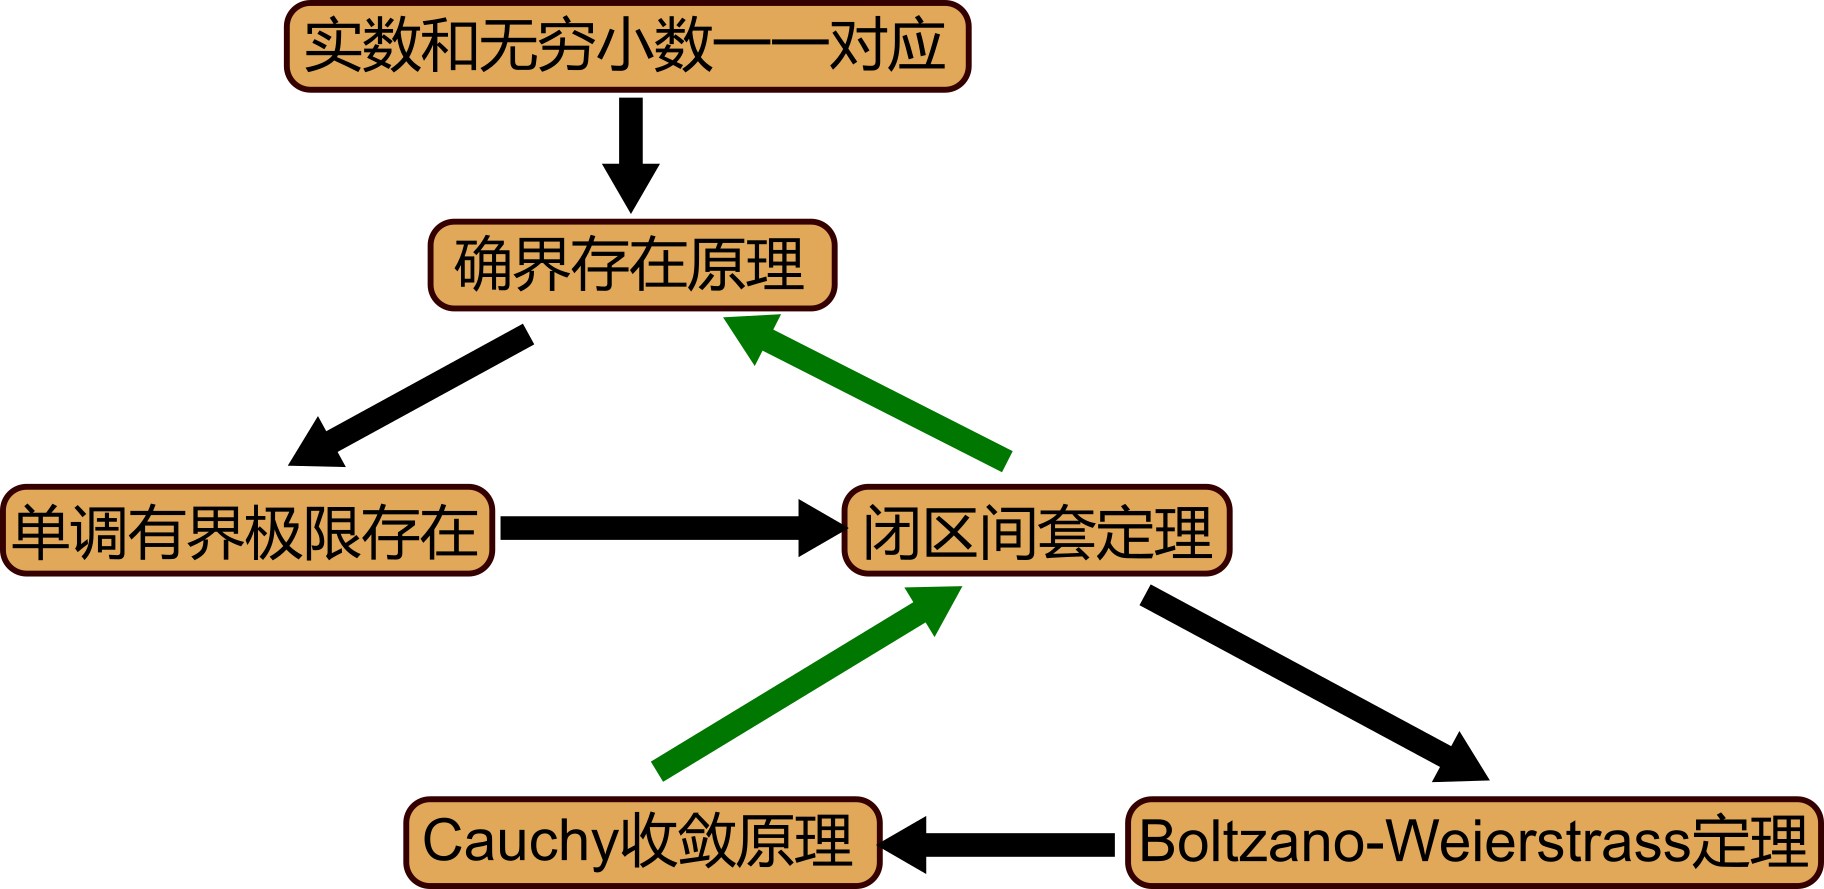
\includegraphics[width=0.7\linewidth]{theorem-relation.png}
    \caption{陈老视频中, 实数系定理的关系}
\end{figure}

\chapter{函数极限与连续函数}
% 陈老视频22
函数极限

\[ \funclim{x}{0}{\frac{\sin x}{x}} = 1 \]
\begin{definition}
    $y = f(x)$在$O(x_0, \rho) \backslash \collect{x_0}$上有定义, 如果存在一个数A, 使得对任意给定的$\epsilon > 0$, 可以找到$\delta > 0$, 当$0 < \left| x - x_0 \right| < \delta$时, 成立$\left| f(x) - A\right| < \epsilon$, 则称A是$f(x)$在$x_0$点的极限,记为$\lim_{x \to x_0} f(x) = A$或者$f(x) \to A (x \to x_0)$。如果不存在满足上述性质的A, 则称$f(x)$在$x_0$点极限不存在。
\end{definition}
$O(x_0, \rho) \backslash \collect{x_0}$称为去心邻域。

% 陈老视频23
\begin{proposition}
    证明:
    \[ \funclim{x}{0}{e^x} = 1\]
\end{proposition}
\begin{proof}

\end{proof}

\begin{proposition}
    证明:
    \[ \funclim{x}{2}{x^2} = 4 \]
\end{proposition}
\begin{proof}

\end{proof}

\begin{proposition}
    证明:
    \[ \funclim{x}{1}{\frac{x(x-1)}{x^2-1}} = \frac{1}{2} \]
\end{proposition}
\begin{proof}
    
\end{proof}

函数极限的性质
\begin{theorem}[函数极限的唯一性]
    设A, B都是$f(x)$在$x_0$的极限, 则$A=B$。 
\end{theorem}
\begin{proof}
    证明类似证明数列极限的唯一性
\end{proof}

\begin{theorem}[函数极限的局部保序性]
    若$\funclim{x}{x_0}{f(x)} = A, \funclim{x}{x_0}{g(x)} = B, A > B$, 则$\exists \delta > 0$, 当x有$0 < \left| x - x_0 \right| < \delta $时, $f(x) > g(x)$  
\end{theorem}
\begin{proof}
    证明类似证明数列极限的保序性
\end{proof}

\begin{lemma}
    $\funclim{x}{x_0}{f(x)} = A \neq 0$, 则$\exists \delta > 0$, $\forall x ( 0 < \left| x - x_0\right| < \delta)$, $\left| f(x) \right| > \frac{\left| A \right|}{2}$。
\end{lemma}
\begin{proof}
    请使用局部保序性证明
\end{proof}

\begin{lemma}
    假设$\funclim{x}{x_0}{f(x)} = A, \funclim{x}{x_0}{g(x)} = B$, 若$\exists \delta > 0, \forall x (x < \left| x - x_0\right| < \delta)$, 有$f(x) \ge g(x)$, 则$A \ge B$
\end{lemma}
\begin{proof}

\end{proof}

% 陈老视频24

\begin{theorem}[函数极限的局部有界性]
    若$\funclim{x}{x_0}{f(x)} = A$, 则$\exists \delta$, $\forall x(0 < \left| x - x_0 \right| < \delta)$, $m \le f(x) \le M$, m, M为固定实数。

    若$f(x)$在$x_0$有定义, 则在$x$满足$\left| x - x_0 \right| < \delta$的条件下, $\min\{m, f(x)\} \le f(x) \le \max\{M, f(x)\}$。
\end{theorem}
\begin{proof}
    请使用局部保序性证明
\end{proof}

\begin{theorem}[函数极限的夹逼性定理]
    若$\exists r > 0$, $\forall x(x < \left| x - x_0 \right| < r)$, 有$g(x) \le f(x) \le h(x)$, 且$\funclim{x}{x_0}{g(x)} = \funclim{x}{x_0}{h(x)} = A$, 则$\funclim{x}{x_0}{f(x)} = A$
\end{theorem}
\begin{proof}
    
\end{proof}

\begin{proposition}
    证明: 
    \[ \funclim{x}{0}{\frac{\sin x}{x}} = 1 \]
\end{proposition}
\begin{proof}
    使用夹逼性证明。

    再用数列逼近证明。
\end{proof}

\begin{theorem}[函数极限四则运算]
    假设$\funclim{x}{x_0}{f(x)} = A$, $\funclim{x}{x_0}{g(x)} = B$, 则: 
    \begin{enumerate}
        \item $\funclim{x}{x_0}{\alpha f(x) + \beta g(x)} = \alpha A + \beta B$
        \item $\funclim{x}{x_0}{f(x)g(x)} = AB$
        \item $\funclim{x}{x_0}{\frac{f(x)}{g(x)}} = \frac{A}{B}(B \neq 0)$
    \end{enumerate}
\end{theorem}
\begin{proof}
    
\end{proof}

\begin{proposition}
    求:
    \[ \funclim{x}{0}{\frac{\sin \alpha x}{x}} \]
    的极限。
\end{proposition}
\begin{proof}
\end{proof}

\begin{proposition}
    求:
    \[ \funclim{x}{0}{\frac{\sin \alpha x}{\sin \beta x}} \]
    的极限。
\end{proposition}
\begin{proof}
    
\end{proof}

% 陈老视频25
\section{函数极限和数列极限的关系}
\begin{theorem}[否定命题的分析表示]
    $\collect{x_n}$以$a$为极限: $\forall \epsilon > 0$, $\exists N$, $\forall n > N$, $\left| x_n - a \right| < \epsilon$。

    $\collect{x_n}$不以$a$为极限: $\exists \epsilon > 0$, $\forall N$, $\exists n > N$, $\left| x_n - a \right| \ge \epsilon$
\end{theorem}
\begin{theorem}[heine定理]
    $\funclim{x}{x_0}{f(x)} = A$存在的充分必要条件是: 对于任意的满足$x_n \neq x_0$, $\mylim{n}{x_n} = x_0$的数列$\collect{x_n}$, $\collect{f(x_n)}$收敛于A。
\end{theorem}
\begin{proof}
    {\bf 证明必要性}, 即证明: 
    
    若$\funclim{x}{x_0}{f(x)} = A$, 则对于任意的满足$x_n \neq x_0$, $\mylim{n}{x_n} = x_0$的数列$\collect{x_n}$, $\collect{f(x_n)}$收敛于A。

    因为$\funclim{x}{x_0}{f(x)} = A$, 则$\forall \epsilon > 0$, $\exists \delta > 0$, $\forall x ( 0 < \left| x - x_0 \right| < \delta)$, 成立$\left| f(x) - A \right| < \epsilon$。

    又因为对于$\collect{x_n}$, 有$x_n \neq x_0$且$\mylim{n}{x_n} = 0$, 即$\forall \delta > 0$, $\exists N \in \mathbb{N}^+$, $\forall n > N$, 成立$0 < \left| x_n - x_0 \right| < \delta$。

    则$\forall \epsilon > 0$, $\exists \delta > 0$, 对于该$\delta$, $\exists N \in \mathbb{N}^+$, $\forall n > N$, 有$0 < \left| x_n - x_0 \right| < \delta$, 且在该$\delta$下有$\left| f(x_n) - A \right| < \epsilon$。

    \qed

    {\bf 证明充分性}, 即证明:
    
    若对于任意的满足$x_n \neq x_0$, $\mylim{n}{x_n} = x_0$的数列$\collect{x_n}$, $\collect{f(x_n)}$收敛于A, 则$\funclim{x}{x_0}{f(x)} = A$。

    利用反证法, 若$\funclim{x}{x_0}{f(x)} \neq A$, 则$\exists \epsilon_0 > 0$, $\forall \delta > 0$, $\exists x ( 0 < \left| x - x_0 \right| < \delta)$, 使得$\left| f(x) - A \right| \ge \epsilon_0$

    取$\delta_n = \frac{1}{n}, n = 1, 2, 3, \cdots$,则对于$\epsilon_0$,有:
    \begin{gather*}
        \exists x_1(0 < \left| x_1 -x_0 \right| < 1), \left| f(x_1) - A \right| \ge \epsilon_0 \\
        \exists x_2(0 < \left| x_2 -x_0 \right| < \frac{1}{2}), \left| f(x_2) - A \right| \ge \epsilon_0 \\
        \exists x_3(0 < \left| x_3 -x_0 \right| < \frac{1}{3}), \left| f(x_3) - A \right| \ge \epsilon_0 \\
        \cdots \cdots
    \end{gather*}
    对于数列$\collect{x_n}$, 对于$\epsilon_0$, $\forall n$, $\left| f(x_n) - A\right| \ge \epsilon_0$恒成立。

    即: $\exists \epsilon = \epsilon_0 > 0$, $\forall N \in \mathbb{N}^+$, $\exists n > N$, $\left| f(x_n) - A\right| > \epsilon$。
    则存在数列$\collect{x_n}$不收敛于A。这与条件矛盾, 则假设不成立。

    \qed

\end{proof}

\begin{proposition}
    $f(x) = \sin \frac{1}{x}$在$x_0 = 0$处极限不存在。
\end{proposition}
\begin{proof}
    
\end{proof}

\begin{lemma}
    $\funclim{x}{x_0}{f(x)}$存在并且有限(收敛)的充分必要条件是: 对任意满足$x_n \neq x_0$, $\mylim{n}{x_n} = x_0$的$\collect{x_n}$, $\collect{f(x_n)}$收敛。
\end{lemma}
\begin{proof}
    
\end{proof}

\section{单侧极限}
\begin{definition}
    假设$f(x)$在$(x_0 - \rho, x_0)$有定义, 如果存在B, $\forall \epsilon > 0$, $\exists \delta > 0$, $\forall x(-\delta < x-x_0 < 0)$, 成立$\left| f(x) - B\right| < \epsilon$, 则称B是$f(x)$在$x_0$的左极限, 记为$\funclim{x}{x_0^-}{f(x)} = B(f(x)\to B(x \to x_0^-))$。

    类似地, 假如存在C, $\exists \epsilon > 0$, $\exists \delta > 0$, $\forall x(0 < x - x_0 < \delta )$, 成立$\left| f(x) - C \right| < \epsilon$, 则称C是$f(x)$在$x_0$的右极限, 记为$\funclim{x}{x_0^+}{f(x)} = C(f(x)\to C(x \to x_0^+))$。

    则$\funclim{x}{x_0}{f(x)} = A \Leftrightarrow \funclim{x}{x_0^-}{f(x)} = \funclim{x}{x_0^+}{f(x)} = A$
\end{definition}

\begin{proposition}
    \begin{equation*}
        \mathrm{sign} (x) = \left\{ 
            \begin{aligned}
                -1 \quad x < 0 \\
                0 \quad x = 0 \\
                1 \quad x > 0 
            \end{aligned}
        \right.
    \end{equation*}
\end{proposition}
\begin{proof}
    
\end{proof}
\begin{proposition}
    \begin{equation*}
        f(x) = \left\{
            \begin{aligned}
               \frac{\sin 2x}{x} \quad x < 0 \\
               2\cos(x^2) \quad x \ge 0 
            \end{aligned}
        \right.
    \end{equation*}
\end{proposition}

% 陈老视频26
\section{函数极限定义的扩充}
可以将自变量$x$的趋向扩充成以下六种:
\begin{enumerate}
    \item $x \to x_0$
    \item $x \to x_0^+$
    \item $x \to x_0^-$
    \item $x \to +\infty$
    \item $x \to -\infty$
    \item $x \to \infty$
\end{enumerate}
而应变量$f(x)$的趋向可以扩充成以下四种:
\begin{enumerate}
    \item $f(x) \to A$
    \item $f(x) \to +\infty$
    \item $f(x) \to -\infty$
    \item $x \to \infty$
\end{enumerate}
现在加上对应的分析表述, 对于自变量$x$:
\begin{enumerate}
    \item $x \to x_0: \exists \delta > 0, \forall x(0 < \left| x - x_0 \right| < \delta)$
    \item $x \to x_0^+: \exists \delta > 0, \forall x(0 < x - x_0 < \delta)$
    \item $x \to x_0^-: \exists \delta > 0, \forall x(-\delta < x - x_0 < 0)$
    \item $x \to +\infty: \exists X > 0, \forall x(x > X)$
    \item $x \to -\infty: \exists X > 0, \forall x(x < -X)$
    \item $x \to \infty: \exists X > 0, \forall x(\left| x \right| > X)$
\end{enumerate}
对于应变量$f(x)$: 
\begin{enumerate}
    \item $f(x) \to A: \forall \epsilon > 0, \cdots,\left| f(x) - A \right| < \epsilon$
    \item $f(x) \to +\infty: \forall G > 0, \cdots, f(x) > G$
    \item $f(x) \to -\infty: \forall G > 0, \cdots, f(x) < -G$
    \item $x \to \infty: \forall G > 0, \cdots, \left| f(x) \right| > G$
\end{enumerate}

\begin{proposition}
    写出:
    \[ \funclim{x}{x_0^+}{f(x)} = \infty \]
    的分析表述。
\end{proposition}
\begin{proof}
    
\end{proof}
\begin{proposition}
    写出:
    \[ \funclim{x}{+\infty}{f(x)} = A \]
    的分析表述。
\end{proposition}
\begin{proof}
    
\end{proof}
\begin{proposition}
    写出:
    \[ \funclim{x}{-\infty}{f(x)} = +\infty \]
    的分析表述。
\end{proposition}
\begin{proof}
    
\end{proof}

\begin{proposition}
    证明:
    \[ \funclim{x}{-\infty}{e^x} = 0\]
\end{proposition}
\begin{proof}
    
\end{proof}

\begin{proposition}
    证明
    \[ \funclim{x}{1^-}{\frac{x^2}{x-1}} = -\infty \]
\end{proposition}
\begin{proof}
    
\end{proof}

我们讲了函数极限的性质和函数极限的四则运算。讲函数极限的性质的时候是对于收敛函数来讨论的。对于扩充后的函数极限则不一定成立, 特别对于$\infty$。性质要排除$\infty$, 四则运算要排除待定型。

对于扩充后的heine定理应该如何书写:
$\funclim{x}{+\infty}{f(x)} = A$充分必要条件: 对任意的满足$x_n\to +\infty(n \to \infty)$的数列$\collect{x_n}$,, 成立$\collect{f(x_n)}$收敛于A。

$\funclim{x}{+\infty}{f(x)}$存在且有限的充分必要条件是: 对任意满足$x_n \to +\infty(n \to +\infty)$的数列$\collect{x_n}$, $\collect{f(x_n)}$收敛。

% 陈老视频27
\begin{proposition}
    设:
    \[f(x) = \frac{a_n x^n+a_{n-1}x^{n-1}+\cdots+a_k x^k}{b_m x^m+b_{m-1} x^{m-1}+\cdots+b_j x^j} (a_n, a_k \neq 0, b_m, b_j \neq 0)\]
    考虑$\funclim{x}{\infty}{f(x)}$和$\funclim{x}{0}{f(x)}$。
\end{proposition}
\begin{proof}
    $x\to \infty$的情况:

    分三种情况讨论:
    \begin{enumerate}
        \item $n = m$:
        \item $n > m$:
        \item $n < m$:
    \end{enumerate}

    $x \to 0$的情况:

    分三种情况讨论:
    \begin{enumerate}
        \item $k = j$:
        \item $k > j$:
        \item $k < j$:
    \end{enumerate}
\end{proof}

\begin{proposition}
    证明:
    \[ \funclim{x}{\infty}{\left(1+\frac{1}{x}\right)^x} = e\]
\end{proposition}
\begin{proof}
    提示: 夹逼法。
    同时$\funclim{x}{\infty}{\left(1-\frac{1}{x}\right)^x} = \frac{1}{e}$
\end{proof}

函数极限的Cauchy收敛原理

回忆以下数列的情况:
$\mylim{n}{x_n}$收敛$\Longleftrightarrow$ $\forall \epsilon > 0, \exists N, \forall n, m > N, \left| x_n - x_m \right| < \epsilon$。

在函数中, 我们做了拓广, 并不是所有的拓广都有Cauchy收敛原理。

对于函数发散时是没有Cauchy收敛原理的。
\begin{theorem}[函数极限的Cauchy收敛原理]
    $\funclim{x}{+\infty}{f(x)}$存在并且有限(收敛)$\Longleftrightarrow$ $\forall \epsilon > 0, \exists X > 0, \forall x', x'' > X, \left| f(x') - f(x'') \right| < \epsilon$ 
\end{theorem}
\begin{proof}
    
\end{proof}

% 陈老视频28
\section{连续函数}
分析上讲, $f(x)$在$x_0$点连续: 当$x \to x_0$时, $f(x) \to f(x_0)$。
\begin{definition}
    设$f(x)$在$x_0$的某个邻域中有定义, 且成立
    \[ \funclim{x}{x_0}{f(x)} = f(x_0) \]
    则称$f(x)$在$x_0$点连续,$x_0$是$f(x)$的连续点。

    符号表述:
    $\forall \epsilon > 0$, $\exists \delta > 0$, $\forall x(\left| x - x_0 \right| < \delta)$, 成立$\left| f(x) - f(x_0) \right| < \epsilon$。
\end{definition}

开区间情况:
\begin{definition}
    若$f(x)$在$(a, b)$的每一点上都连续, 则称$f(x)$在开区间$(a, b)$上连续。
\end{definition}
\begin{proposition}
    证明:
    \[ f(x) = \frac{1}{x}\]
    在$(0, 1)$连续。
\end{proposition}
\begin{proof}
    
\end{proof}

闭区间情况:
\begin{definition}
    若$\funclim{x}{x_0^-}{f(x)} = f(x_0)$, 则称$f(x)$在$x_0$点左连续。

    若$\funclim{x}{x_0^+}{f(x)} = f(x_0)$, 则称$f(x)$在$x_0$点右连续。

    符号表示:

    {\bf 左连续}: $\forall \epsilon > 0$, $\exists \delta > 0$, $\forall x(-\delta < x-x_0 \le 0)$: $\left| f(x) - f(x_0)\right| < \epsilon$。

    {\bf 右连续}: $\forall \epsilon > 0$, $\exists \delta > 0$, $\forall x(0 \le x-x_0 < \delta)$: $\left| f(x) - f(x_0)\right| < \epsilon$。   
\end{definition}

\begin{definition}
    $f(x)$在$(a, b)$上连续, 且在a点右连续, 在b点左连续, 则称$f(x)$在闭区间$[a, b]$上连续。
\end{definition}
\begin{proposition}
    证明:
    \[ f(x) = \sqrt{x(1-x)}\]
    在$(0, 1)$闭区间上连续。
\end{proposition}
\begin{proof}
    
\end{proof}

注:关于函数$f(x)$在一个区间里面连续, 整合以上的定义。
\begin{definition}
    设$f(x)$定义在某区间X上, 若$\forall x_0 \in X$, 及$\forall \epsilon > 0$, $\exists \delta > 0$, $\forall x \in X(\left|x - x_0 \right|<\delta)$, $\left| f(x) - f(x_0) \right| < \epsilon$。则称$f(x)$在区间X上连续。
\end{definition}
\begin{proposition}
    证明:
    \[ f(x) = \sin(x)\]
    在$(-\infty, +\infty)$上连续。
\end{proposition}
\begin{proof}
    同理$f(x) = \cos(x)$在$(-\infty, +\infty)$上连续。
\end{proof}

% 陈老视频29
\begin{proposition}
    证明:
    \[ f(x) = a^x (a > 0, a \neq 1)\]
    在$(-\infty, +\infty)$上连续。
\end{proposition}
\begin{proof}
    
\end{proof}
\section{连续函数的四则运算}
\begin{theorem}
    有$\funclim{x}{x_0}{f(x)} = f(x_0)$, $\funclim{x}{x_0}{g(x)} = g(x_0)$, 则:
    \begin{enumerate}
        \item $\funclim{x}{x_0}{\alpha f(x) + \beta g(x)} = \alpha f(x_0) + \beta g(x_0)$
        \item $\funclim{x}{x_0}{f(x)g(x)} = f(x_0)g(x_0)$
        \item $\funclim{x}{x_0}{\frac{f(x)}{g(x)}} = \frac{f(x_0)}{g(x_0)}(g(x_0) \neq 0)$
    \end{enumerate}
\end{theorem}

\begin{proposition}
    求:
    \[ \funclim{x}{2}{\frac{x^2+\sin x}{3^x+2x}}\]
\end{proposition}
\begin{proof}
    
\end{proof}

\begin{proposition}
    \[ P_n(x) = a_n x^n + a_{n-1} x^{n-1} + \cdots + a_0\]
    \[ Q(x) = \frac{a_n x^n + a_{n-1} x^{n-1} + \cdots + a_0}{b_m x^m + b_{m-1} x^{m-1} + \cdots + b_0}\]
\end{proposition}
\begin{proof}
    $f(x) = c, g(x) = x$
\end{proof}

\begin{proposition}
    已知$\sin(x)$, $\cos(x)$在$(-\infty, +\infty)$上连续。

    $\tan(x) = \frac{\sin(x)}{\cos(x)}$, 在$\left\{ x\left| x \neq k\pi + \frac{\pi}{2}, k \in \mathbb{Z}\right.\right\}$上连续。

    $\cot(x) = \frac{\cos(x)}{\sin(x)}$, 在$\left\{ x\left| x \neq k\pi, k \in \mathbb{Z}\right.\right\}$上连续。
\end{proposition}
\begin{proof}
    
\end{proof}

\section{不连续点的类型}
连续的定义:$\funclim{x}{x_0}{f(x)} = f(x_0)$

该定义包含了如下几层意思:
\begin{enumerate}
    \item $f(x)$在$x_0$点有定义。
    \item $\funclim{x}{x_0^+}{f(x)} = f(x_0)$ 
    \item $\funclim{x}{x_0^-}{f(x)} = f(x_0)$
\end{enumerate}
\subsection{第一类不连续点}
$\funclim{x}{x_0^+}{f(x)} \neq \funclim{x}{x_0^-}{f(x)}$
\begin{proposition}
    \begin{equation*}
        \mathrm{sign} (x) = \left\{ 
            \begin{aligned}
                -1 \quad x < 0 \\
                0 \quad x = 0 \\
                1 \quad x > 0 
            \end{aligned}
        \right.
    \end{equation*}
    在$x=0$不连续。
\end{proposition}
称第一类不连续点为跳跃点。
\subsection{第二类不连续点}
$\funclim{x}{x_0^+}{f(x)}$和$\funclim{x}{x_0^-}{f(x)}$至少有一个不存在。
\begin{proposition}
    $f(x) = \sin(\frac{1}{x})$,$x=0$是它的第二类不连续点。
\end{proposition}
\begin{proof}
    
\end{proof}
\begin{proposition}
    $f(x) = e^{\frac{1}{x}}$, $x = 0$是它的第二类不连续点。
\end{proposition}
\begin{proof}
    
\end{proof}
\subsection{第三类不连续点}
\begin{equation*}
    \funclim{x}{x_0^+}{f(x)} = \funclim{x}{x_0^-}{f(x)}\left\{
    \begin{aligned}
        & \neq f(x_0) \\
        & f(x)\text{在}x_0\text{点没定义。} 
    \end{aligned}
    \right.
\end{equation*}

\begin{proposition}
    $f(x) = x\sin(\frac{1}{x})$, 在$x=0$极限存在, 但是没有定义。
\end{proposition}
\begin{proof}
    
\end{proof}
第三类不连续点称为可去不连续点。
\begin{proposition}
    \begin{equation*}
        \mathrm{D}(x) = \left\{
            \begin{aligned}
                &1 \quad x\text{是有理数} \\
                &0 \quad x\text{是无理数}
            \end{aligned}
        \right.
    \end{equation*}
    Dirichlet函数属于第二类不连续点。
\end{proposition}
\begin{proof}
    
\end{proof}

% 陈老视频30
\begin{proposition}
    黎曼(Riemann)函数:
    \begin{equation*}
        \mathrm{R}(x) = \left\{
            \begin{aligned}
                &0 \quad x\text{是无理数} \\
                &\frac{1}{p} \quad x=\frac{q}{p}, p \in \mathbb{N}^+, q \in \mathbb{Z}\backslash\{0\}, p,q\text{互质} \\
                &1 \quad x = 0
            \end{aligned}
            \right.
    \end{equation*}
    $\forall x_0 \in (-\infty, +\infty)$, $\funclim{x}{x_0}{\mathrm{R}(x)} = 0$。即$\mathrm{R}(x)$在一切无理点连续, 在一切有理点不连续。
\end{proposition}
为什么定义0的时候是1? 因为1可以写成$\frac{0}{1}$, 并且Riemann函数有周期性, 为了保持周期性, 因此定义0的时候是1。
\begin{proof}
    
\end{proof}

\begin{proposition}
    区间$(a, b)$上的单调函数的不连续点必为第一类。    
\end{proposition}
\begin{proof}
    
\end{proof}
\section{反函数}
映射: $f: X \to Y$ 为单射, 则$\exists f^{-1}: R_f \to X$。

存在性、连续性、可导性(可导性暂时不讲)

严格单调增加:$\forall x_1 < x_2 \Rightarrow f(x_1) < f(x_2)(y_1 < y_2)$, 即$x_1 \neq x_2, y_1 \neq y_2$。
\begin{theorem}[反函数存在定理]\label{theorem:inverse-func-exists}
    若$f(x)$在$D_f$上严格单调增加(减少), 则存在f的反函数$f^{-1}(y)$, $y \in R_f $,且$f^{-1}$也严格单调增加(减少)。
\end{theorem}
\begin{proof}
    
\end{proof}

% 陈老视频31
\begin{theorem}[反函数连续性定理]
    假设$y = f(x)$在$[a, b]$上连续且严格单调增加, 设$f(a)=\alpha$, $f(b)=\beta$, 则反函数在$[\alpha, \beta]$上连续。
\end{theorem}
\begin{proof}
    
\end{proof}

\begin{proposition}
    $y = \sin(x)$, $y = \arcsin(x)$

    $y = \cos(x)$, $y = \arccos(x)$

    $y = \tan(x)$, $y = \arctan(x)$
\end{proposition}
\begin{proof}
    
\end{proof}
\begin{proposition}
    $y = a^x(a > 0, a \neq 1)$, $y = \log_a(x)$

    $y = x^n, n \in \mathbb{Z}$

    $y = x^\alpha = e^{\ln x^\alpha} = e^{\alpha \ln x}$
\end{proposition}
\begin{proof}
    
\end{proof}

讨论一个问题, $\funclim{u}{u_0}{f(x)} = A$, $\funclim{x}{x_0}{g(x)} = u_0$

那么$\funclim{x}{x_0}{f\circ g(x)}$是否等于A?

反例:
\begin{equation*}
    f(u) = \left\{
        \begin{aligned}
            0 & \quad u = 0 \\
            1 & \quad u \neq 0 \\
        \end{aligned}
    \right.
\end{equation*}
\begin{equation*}
    g(x) = x\sin\left(\frac{1}{x}\right)
\end{equation*}
则复合起来为:
\begin{equation*}
    f\circ g(x) \left\{
        \begin{aligned}
           0 & \quad x = \frac{1}{n\pi} \\
           1 & \quad x \neq \frac{1}{n\pi} 
        \end{aligned}
    \right.
\end{equation*}
\begin{theorem}
    $u = g(x)$在$x_0$连续, $g(x_0) = u_0$, $f(u)$在$u_0$连续。则$f\circ g$在$x_0$连续。
\end{theorem}
\begin{proof}
    
\end{proof}


\begin{proposition}
    \[ \sh(x) = \frac{e^x-e^{-x}}{2}, \ch(x) = \frac{e^x+e^{-x}}{2} \]
\end{proposition}
\begin{proof}
    
\end{proof}

% 陈老视频32
\begin{proposition}
    对任意实数$\alpha$, $f(x) = x^\alpha$在$(0, +\infty)$上连续。
\end{proposition}
\begin{proof}
    
\end{proof}

\begin{theorem}
    一切初等函数在它的定义域上连续。
\end{theorem}

\begin{proposition}
    \[ \funclim{x}{0}{\left(\cos x\right)^{\frac{1}{x^2}}} \]
\end{proposition}
\begin{proof}
    
\end{proof}

\begin{proposition}
    放射性物质的质量变化:

    设$t = 0$时,物质的总量为$M = M(0)$, 放射的比例系数为k, 求时刻t的时候, $M(t)$为多少?
\end{proposition}
\begin{proof}
    
\end{proof}

% 陈老视频33
\section{无穷小量与无穷大量的阶}
无穷小量的阶:

在数列极限的时候, 我们提及:$\mylim{n}{x_n} = 0$, $\collect{x_n}$---无穷小量。

对于函数极限:
$\funclim{x}{x_0}{f(x)} = 0$, 则称当$x \to x_0$时, $f(x)$是无穷小量。

当$x \to x_0$, $u(x)$, $v(x)$都是无穷小量。

\begin{definition}
    $\funclim{x}{x_0}{\frac{u(x)}{v(x)}} = 0$, 则称当$x \to x_0$时, $u(x)$是$v(x)$的高阶无穷小量, 记为$u(x) = o(v(x)), (x \to x_0)$。    
\end{definition}

\begin{proposition}
    \[ \funclim{x}{x_0}{\frac{1-\cos(x)}{x}}\] 
\end{proposition}
\begin{proof}
    
\end{proof}

\begin{proposition}
    \[ \funclim{x}{0}{\frac{\tan(x) - \sin(x)}{x^2}} \]
\end{proposition}
\begin{proof}
    
\end{proof}
\begin{definition}
    若存在$A > 0$, 当$x$在$x_0$的某一去心邻域中$\collect{x|  0 < \left| x - x_0\right| < \rho}$,成立 $\left| \frac{u(x)}{v(x)} \right| \le A$, 则称当$x \to x_0$时, $\frac{u(x)}{v(x)}$是有界量, 记为$u(x) = O(v(x)), (x \to x_0)$。    
\end{definition}

\begin{proposition}
    \[u(x) = x\sin\left(\frac{1}{x}\right), u(x) = O(v(x))\]
\end{proposition}
\begin{proof}
    
\end{proof}

\begin{definition}
    若$\exists 0 < a < A < +\infty$, 在$\collect{x|  0 < \left| x - x_0\right| < \rho}$中, $0 < a \le \left| \frac{u(x)}{v(x)} \right| \le A < +\infty$, 则称$u(x)$, $v(x)$在$x \to x_0$时是同阶无穷小量。
\end{definition}

\begin{proposition}
    \[ u(x) = x(1+\sin\left( \frac{1}{x} \right)), v(x) = x, (x \to 0) \]
\end{proposition}
\begin{proof}
    
\end{proof}

\begin{proposition}
    \[ u(x) = x(2+\sin\left( \frac{1}{x} \right)), v(x) = x, (x \to 0) \]
\end{proposition}

\begin{definition}
    若$\funclim{x}{x_0}{\frac{u(x)}{v(x)}} = 1$, 则称当$x \to x_0$时, $u(x)$与$v(x)$是等价无穷小量, 记为$u(x)\sim v(x), (x \to x_0)$。
\end{definition}
\begin{proposition}
    \[ \funclim{x}{0}{\frac{\sin(x)}{x}} = 1, \sin(x) \sim x(x \to x_0)\]
\end{proposition}
\begin{proof}
    
\end{proof}
\begin{proposition}
    \[ \funclim{x}{0}{\frac{1- \cos(x)}{\frac{1}{2}x^2}} \]
\end{proposition}
\begin{proof}
    
\end{proof}
\begin{proposition}
    \[ \funclim{x}{0}{\frac{\tan(x) - \sin(x)}{\frac{1}{2}x^3}} \]    
\end{proposition}

注:(1) 取$v(x) = (x - x_0)^k$可知$u(x)$是几阶的无穷小量。

(2)$x \to 0^+$, $\frac{-1}{\ln (x)}$是正无穷小量。对任意的$\alpha > 0$, $\frac{-1}{\ln (x)}$是$x^\alpha$的低阶无穷小量, 即:
\[ \funclim{x}{0^+}{\frac{\frac{-1}{\ln (x)}}{x^\alpha}} = +\infty\]
这时候, 记$\frac{-1}{\ln (x)} = o(1), (x \to 0^+)$

又比如$u(x) = \sin\left( \frac{1}{x}\right)(x \to 0)$, 不是无穷小量但是是有界量, 则记为$u(x) = O(1), (x \to 0)$。

无穷大量的阶: 

$\funclim{x}{x_0}{f(x)} = \infty (+\infty, -\infty)$, 则称当$x \to x_0$时, $f(x)$是(正, 负)无穷大量。

\begin{definition}
    假设$u(x)$, $v(x)$当$x \to x_0$时都是无穷大量, 若$\funclim{x}{x_0}{\frac{u(x)}{v(x)}} = \infty$, 这说明当$x \to x_0$时, $u(x)$是$v(x)$的高阶无穷大量。
\end{definition}

% 陈老视频34
$n^n >> n! >> a^n(a > 1) >> n^\alpha(\alpha > 0) >> \ln^\beta(n)(\beta > 0)$

\begin{proposition}
    设$a > 1$, k是正整数, 求: 
    \[ \funclim{x}{+\infty}{\frac{a^x}{x^k}} \]
    \[ \funclim{x}{+\infty}{\frac{\ln^k(x)}{x}}\]
\end{proposition}
\begin{definition}
    若存在$A > 0$, 在$\collect{x | 0 < \left| x - x_0\right| < \rho}$, 成立:
    \[ \left| \frac{u(x)}{v(x)} \right| \le A \]
    则称当$x \to x_0$时, $\frac{u(x)}{v(x)}$是有界量, 记为$u(x) = O(v(x)), (x \to x_0)$
\end{definition}

\begin{definition}
    若存在$0 < a < A < +\infty$, 在$\collect{x | 0 < \left| x - x_0\right| < \rho}$, 成立:
    \[ 0 < a \le \left| \frac{u(x)}{v(x)} \right| \le A < +\infty \]
    则称当$x \to x_0$时, $u(x)$, $v(x)$是同阶无穷大量。
\end{definition}
若$\funclim{x}{x_0}{\frac{u(x){v(x)}}} = c \neq 0$, 则$u(x)$, $v(x)$一定是同阶无穷大量。
\begin{definition}
    若$\funclim{x}{x_0}{\frac{u(x)}{v(x)}} = 1$, 则称$u(x)$与$v(x)$是等价无穷大量, 记为$u(x) \sim v(x), (x \to x_0)$。
\end{definition}

\begin{proposition}
    \[ u(x) = x^3\sin \left( \frac{1}{x} \right), v(x) = x^2\]
\end{proposition}
\begin{proof}
    
\end{proof}
\begin{proposition}
    \[ \funclim{x}{\frac{\pi}{2}^-}{\left( \frac{\pi}{2} - x \right)\tan(x)}\]
\end{proposition}
\begin{proof}
    
\end{proof}
当$x \to 0^+$, $\frac{-1}{\ln(x)}$关于$x^\alpha$都是低阶无穷小量。
\begin{proposition}
    $x \to 0^+$, k为任意的正整数,$\left( \frac{-1}{\ln(x)}\right)^k$关于x是低阶无穷小量。
\end{proposition}
\begin{proof}
    
\end{proof}
\begin{proposition}
    当$x \to 0^+$, $e^{-\frac{1}{x}}$关于$x^k$是高阶无穷小量。
\end{proposition}
\begin{proof}
    
\end{proof}

等价量:

$\sin(x) \sim x$
\begin{proposition}
    \[ \ln(1+x) \sim x, (x \to 0) \] 
\end{proposition}
\begin{proof}
    
\end{proof}
\begin{proposition}
    \[ e^x - 1 \sim x, (x \to 0)\]
\end{proposition}
\begin{proof}
    
\end{proof}
\begin{proposition}
    \[ \left( 1 + x\right)^\alpha \sim \alpha x, (x \to 0)\]
\end{proposition}
\begin{proof}
    
\end{proof}
\begin{proposition}
    \[ u(x) = \sqrt{x + \sqrt{x}}\]
    讨论$x \to +\infty$和$x \to 0^+$时的阶数。
\end{proposition}
\begin{proof}
    
\end{proof}
\begin{proposition}
    \[ v(x) = 2x^3 + 3x^5\]
    讨论$x \to \infty$和$x \to 0$时的阶数。
\end{proposition}
\begin{proof}
    
\end{proof}

% 陈老视频35
\begin{theorem}
    $u(x)$, $v(x)$, $w(x)$在$x_0$的某个去心邻域上有定义, 且
    \[ \funclim{x}{x_0}{\frac{v(x)}{w(x)}} = 1, v(x) \sim w(x), (x \to x_0)\]
    则
    \begin{enumerate}
        \item $\funclim{x}{x_0}{u(x)w(x)} = A \Longleftrightarrow \funclim{x}{x_0}{u(x)v(x)} = A$
        \item $\funclim{x}{x_0}{\frac{u(x)}{w(x)}} = A \Longleftrightarrow \funclim{x}{x_0}{\frac{u(x)}{v(x)}} = A$
    \end{enumerate}
\end{theorem}

\begin{proposition}
    计算:
    \[ \funclim{x}{0}{\frac{\ln(1+x^2)}{\left(e^{2x}-1\right)\tan(x)}}\]
\end{proposition}
\begin{proof}
    
\end{proof}

\begin{proposition}
    计算:
    \[ \funclim{x}{0}{\frac{\sqrt{1+x}-e^{\frac{x}{3}}}{\ln(1+2x)}}\]
\end{proposition}
\begin{proof}
    
\end{proof}

\begin{proposition}
    计算:
    \[ \funclim{x}{\infty}{x\left(\sqrt[3]{x^3+x}+\sqrt[3]{x^3-x}\right)}\]
\end{proposition}
\begin{proof}
    
\end{proof}

\begin{proposition}
    计算:
    \[ \funclim{x}{0}{\frac{\sqrt{1+x}-1-\frac{x}{2}}{x^2}} \]
\end{proposition}

% 陈老视频36
\section{闭区间上的连续函数}
\begin{theorem}[有界性定理]
    $f(x)$在闭区间$[a, b]$上连续, 则$f(x)$在闭区$[a, b]$上有界。
\end{theorem}
\begin{proof}
    
\end{proof}

\begin{theorem}[最值定理]
    $f(x)$在$[a, b]$上连续, 则$f(x)$必能在$[a, b]$上取到最大值和最小值, 即$\exists \xi, \eta \in [a, b]$, 使得$f(\xi) \le f(x) \le f(\eta), \forall x \in [a, b]$。
\end{theorem}
\begin{proof}
    
\end{proof}

\begin{theorem}[零点存在定理]
    $f(x)$在$[a, b]$上连续, 如果$f(a)f(b) < 0$, 则$\exists \xi \in [a, b]$, 使得$f(\xi) = 0$。
\end{theorem}
\begin{proof}
    
\end{proof}

\begin{proposition}
    \[ p(x) = 2x^3-3x^2-3x+2 \]
\end{proposition}
\begin{proof}
    
\end{proof}

\begin{proposition}
    $f(x)$在$[a, b]$上连续, $f([a, b]) \subset [a, b]$, 则$\exists \xi \in [a, b]$, 使得$f(\xi) = \xi$($\xi$称为$f$的不动点)。
\end{proposition}
\begin{proof}
    
\end{proof}

\begin{proposition}
    $f(x)$在$(a, b)$上连续, $f((a, b)) \subset (a, b)$, 则是否$f$也有不动点?
\end{proposition}
\begin{proof}
    
\end{proof}

% 陈老视频37
\begin{theorem}[中间值定理]
    $f(x)$在闭区间$[a, b]$上连续, 则它一定能取到最大值M与最小值m之间的任何一个值。
\end{theorem}
\begin{proof}
    
\end{proof}

\subsection{一致连续概念}
\begin{definition}
    X是某一区间, $f(x)$在X上连续, 是指$f(x)$在X上的每一点连续(在端点指右或者左连续)。

    分析表述: $\forall x_0 \in X$, $\forall \epsilon > 0$, $\exists \delta > 0$, $\forall x \in X(\left| x - x_0 \right| < \delta)$, $\left| f(x) - f(x_0) \right| < \epsilon$
\end{definition}
$\delta = \delta(\epsilon, x_0)$, 能否找到对一切$x_0$适用的$\delta > 0$?

若能找到这样的$\delta > 0$, 则有:

$\forall \epsilon > 0$, $\exists \delta = \delta(\epsilon) > 0$, $\forall x', x'' \in X(\left| x' - x'' \right| < \delta)$: $\left| f(x') - f(x'') \right| < \epsilon$。

问题: 这样的$\delta(\epsilon) > 0$是否一定能找到?不一定!

存在$\delta(\epsilon) > 0 \Longleftrightarrow \inf_{x_0 \in X}\delta^*(\epsilon, x_0) > 0$ (令所有适用的$\delta(\epsilon, x_0)$中的最大者(或上确界)为$\delta^*(\epsilon, x_0)$)

\begin{definition}[一致连续]
    $f(x)$在区间X上有定义, 假如$\forall \epsilon > 0$,$\exists \delta > 0$, $\forall x', x'' \in X(\left| x' - x'' \right| < \delta)$: $\left| f(x') - f(x'') \right| < \epsilon$, 则称$f(x)$在区间X上一致连续。
\end{definition}
$f(x)$在X上一致连续 $\Rightarrow$ $f(x)$在区间X上连续

\begin{proposition}
    证明:
    \[ y = \sin(x) \]
    在$(-\infty, +\infty)$上一致连续。
\end{proposition}
\begin{proof}
    
\end{proof}

\begin{proposition}
    \[ f(x) = \frac{1}{x} \]
    在区间$(0, 1)$上不是一致连续。
\end{proposition}
\begin{proof}
    
\end{proof}

\begin{theorem}
    假设$f(x)$在区间X上有定义, 则$f(x)$在X上一致连续的充分必要条件是: 对任意点列$x'_n, x''_n \in X$, 只要$\mylim{n}{\left( x'_n - x''_n \right)} = 0$, 则有$\mylim{n}{\left(f(x'_n) - f(x''_n) \right)} = 0$。
\end{theorem}
\begin{proof}
    
\end{proof}

% 陈老视频38
\begin{proposition}
    用以上的定理证明:
    \[ f(x) = \frac{1}{x} \]
    在区间$(0, 1)$上不是一致连续。
\end{proposition}
\begin{proof}
    
\end{proof}

\begin{proposition}
    证明:
    \[  f(x) = \frac{1}{x} \]
    在$(\eta, 1), 0 < \eta < 1$上一致连续。
\end{proposition}

\begin{proposition}
    \[ f(x) = x^2 \]
    在$(0, +\infty)$上非一致连续。
\end{proposition}
\begin{proof}
    
\end{proof}

\begin{proposition}
    \[ f(x) = x^2 \]
    在$(0, A)$上一致连续。
\end{proposition}
\begin{proof}
    
\end{proof}

\begin{theorem}[Cantor定理]
    若$f(x)$在闭区间$[a, b]$连续, 则$f(x)$在$[a, b]$上一致连续。
\end{theorem}
\begin{proof}
    
\end{proof}

\begin{theorem}
    $f(x)$在有限开区间$(a, b)$连续, 则$f(x)$在开区间$(a,b)$上一致连续的充分必要条件是: $f(a^+)$, $f(b^-)$存在。
\end{theorem}
\begin{proof}
    
\end{proof}
% 陈老视频39
\chapter{微分}
\section{微分和导数}
\subsection{微分}
考虑$y = f(x)$, 当$x \to x + \Delta x$时, $f(x) \to f(x+\Delta x)$, 令$\Delta y = f(x+\Delta x) - f(x)$。应该怎么简单地表示$\Delta y$?
\begin{definition}[微分的定义]
    $x_0 \in D_f$, 若存在只与$x_0$有关, 与$\Delta x$无关的$g(x_0)$,使得当$\Delta x \to 0$时:
    \[ \Delta y = g(x_0)\Delta x + o(\Delta x) \]
    则称$f(x)$在$x_0$可微。

    若$f(x)$在区间X的每一点可微, 则称$f(x)$在区间X可微。

    $g(x_0)\Delta x$称为$\Delta y$的线性主要部分。

    $\Delta x \to 0$, 记$\Delta x$为$dx$, 若$f(x)$在$x$点可微, 则有$\Delta y = g(x)\Delta x + o(\Delta x), (\Delta x \to 0)$。则记$\Delta y$为$dy$, 并将上式写为$dy = g(x)dx $。
\end{definition}

\begin{proposition}
    \[ y = f(x) = x^2 \]
    对$\forall x \in (-\infty, +\infty)$, 求微分表示。
\end{proposition}
\begin{proof}
    
\end{proof}

\begin{proposition}
    \[ y = f(x) = \sqrt[3]{x^2} \]
    考虑$f$在$x_0 = 0$是否可微。
\end{proposition}
\begin{proof}
    
\end{proof}

可微$\Rightarrow$连续
\subsection{导数}
$y = f(x)$在$x_0$可微, 则$\Delta y = g(x_0)\Delta x + o(\Delta x), (\Delta x \to 0)$, 那么:
\[ \frac{\Delta y}{\Delta x} = g(x_0) + \frac{o(\Delta x)}{\Delta x} \]
令$\Delta x \to 0$, 则
\[ \funclim{\Delta x}{0}{\frac{\Delta y}{\Delta x}} = g(x_0)\]
\begin{definition}
    设$x_0 \in D_f$, 若极限
    \[ \funclim{\Delta x}{0}{\frac{\Delta y}{\Delta x}} = \funclim{\Delta x}{0}{\frac{f(x+\Delta x) - f(x)}{\Delta x}} \]
    存在, 则称$f(x)$在$x_0$可导, 记这个极限值为$f'(x_0)$(或$y'(x_0)$, $\left.\frac{dy}{dx}\right|_{x = x_0}$, $\left.\frac{df}{dx}\right|_{x = x_0}$)。
\end{definition}
$f(x)$可导的范围是$D_f$的子集, 于是我们可以得到在这子集上的$f(x)$的导函数, 记为$f'(x)$(或$y'(x)$, $\frac{dy}{dx}$, $\frac{df}{dx}$)。

可微$\Rightarrow$可导, 且$f'(x_0) = g(x_0)$。

可导是否一定可微?

可导, 则:
\[ \funclim{\Delta x}{0}{\frac{\Delta y}{\Delta x}} = f'(x_0)\]
则:
\[  \funclim{\Delta x}{0}{\left(\frac{\Delta y}{\Delta x} - f'(x_0) \right)} = 0 \]
\[ \frac{\Delta y}{\Delta x} - f'(x_0) = o(1), (\Delta x \to 0) \]
\[ \Delta y = f'(x_0)\Delta x + o(1)\Delta x \]
\[ \Delta y = f'(x_0)\Delta x + o(\Delta x) \]
即, 可导$\Rightarrow$可微(一元函数下)。

% 陈老视频40
\section{导数的意义与性质}
\begin{proposition}
    抛物线:
    \[ y^2 = 2px \]
    $(x_0, y_0)$是抛物线上一点, 求过$(x_0, y_0)$的切线方程。
\end{proposition}
\begin{proof}
    
\end{proof}

\begin{proposition}
    椭圆:
    \[ \frac{x^2}{a^2} + \frac{y^2}{b^2} = 1 \]
    求椭圆上过$(x_0, y_0)$点的切线。
\end{proposition}
\begin{proof}
    
\end{proof}

% 陈老视频41
$f(x)$在$x_0$处的导数为以下极限:
\[ f'(x_0) = \funclim{\Delta x}{0}{\frac{f(x_0+\Delta x) - f(x_0)}{\Delta x}}\]
称:
\[ f'_+(x_0) = \funclim{\Delta x}{0^+}{\frac{f(x_0+\Delta x) - f(x_0)}{\Delta x}}\]
为$f(x)$在$x_0$的右导数。
称:
\[ f'_-(x_0) = \funclim{\Delta x}{0^-}{\frac{f(x_0+\Delta x) - f(x_0)}{\Delta x}}\]
为$f(x)$在$x_0$的左导数。

因此, $f(x)$在$x_0$可导$\Longleftrightarrow$ $f(x)$在$x_0$的左右导数存在且相等。

以下两个记号不好弄混:$f'_+(x_0)$是$f(x)$在$x_0$的右导数, $f'(x_0^+)$是$f(x)$导数在$x_0$的右极限。

同理, $f'_-(x_0)$是$f(x)$在$x_0$的左导数, $f'(x_0^-)$是$f(x)$导数在$x_0$的左极限。

\begin{proposition}
    $f(x) = \left| x \right|$在$x_0$的左右导数。
\end{proposition}
\begin{proof}
    
\end{proof}

\begin{proposition}
    \begin{equation*}
        f(x) = \left\{ 
            \begin{aligned}
                &x\sin(1/x) &\quad x>0 \\
                &0          &\quad x \le 0
            \end{aligned}
        \right.
    \end{equation*}
    求$f(x)$在$x = 0$的左右导数。
\end{proposition}
\begin{proof}
    
\end{proof}

\begin{proposition}
    \begin{equation*}
        f(x) = \left\{ 
            \begin{aligned}
                & x^2 + b &\quad x > 2 \\
                & ax + 1 &\quad x \le 2
            \end{aligned}
        \right.
    \end{equation*}
    要求确定$a, b$使得$f(x)$在$x_0 = 2$可导。
\end{proposition}
\begin{proof}
    
\end{proof}

$f(x)$在$(a, b)$上每一点可导, 则称$f(x)$在$(a, b)$区间上可导。

$f(x)$在$(a, b)$上每一点可导, 在$x = a$上有右导数, $x = b$又左导数, 则称$f$在闭区间$[a, b]$上可导。

% 陈老视频42
\section{导数四则运算与反函数求导法则}
\begin{proposition}
    求
    \[ y = \sin(x) \]
    的导数。
\end{proposition}
\begin{proof}
    
\end{proof}
同理$y = \cos(x)$, $y'(x) = -\sin(x)$。

\begin{proposition}
    求
    \[ y = \ln(x) \]
    的导数。
\end{proposition}
\begin{proof}
    
\end{proof}

\begin{proposition}
    求
    \[ y = e^x \]
    的导数。
\end{proposition}
\begin{proof}
    
\end{proof}

\begin{proposition}
    求
    \[ y = a^x \]
    的导数。    
\end{proposition}
\begin{proof}
    
\end{proof}

\begin{proposition}
    求
    \[ y = x^\alpha, \alpha \in \mathbb{R} \]
    在定义域$(0, +\infty)$的导数。 
\end{proposition}
\begin{proof}
    
\end{proof}

\begin{theorem}
    若$f$, $g$在同一区间可导, 则$c_1f(x)+c_2g(x)$也在该区间可导, 且有:
    \[ \left(c_1 f(x) + c_2 g(x) \right)' = c_1 f'(x) +c_2 g'(x) \]
\end{theorem}

\begin{theorem}
    若$f$, $g$在同一区间可导, 则$f(x)\dot g(x)$也在该区间可导, 且有:
    \[ \left(f(x) g(x) \right)' = f'(x) g(x) + f(x) g'(x) \]
\end{theorem}
\begin{proof}
    
\end{proof}

\begin{proposition}
    求:
    \[ y = x^3\cos(x) \]
    的导数。
\end{proposition}
\begin{proof}
    
\end{proof}

\begin{proposition}
    求:
    \[ y = \frac{\sin(x)}{x} \]
    的导数。
\end{proposition}
\begin{proof}
    
\end{proof}

\begin{theorem}
    设$g(x)$在某一个区间可导, $g(x) \neq 0$, 则$\frac{1}{g(x)}$也在该区间可导, 且
    \[ \left(\frac{1}{g(x)}\right)' = \frac{-g'(x)}{g^2(x)}\]
\end{theorem}
\begin{proof}
    
\end{proof}

\begin{proposition}
    求:
    \[ y = \sec(x), \left(\sec(x) = \frac{1}{\cos(x)}\right) \]
    的导数。
\end{proposition}
\begin{proof}
    
\end{proof}

\begin{proposition}
    求:
    \[ y = \csc(x), \left( \csc(x) = \frac{1}{\sin(x)} \right) \]
    的导数。
\end{proposition}
\begin{proof}
    
\end{proof}

\begin{lemma}
    $f$, $g$在同一区间可导, $g(x) \neq 0$, 则$\frac{f(x)}{g(x)}$在该区间可导, 且:
    \[ \left( \frac{f(x)}{g(x)} \right)' = \frac{f'(x)g(x)-f(x)g'(x)}{g^2(x)}\]
\end{lemma}
\begin{proof}
    
\end{proof}

\begin{proposition}
    求:
    \[ y = \tan(x) \]
    的导数。
\end{proposition}
\begin{proof}
    
\end{proof}

\begin{proposition}
    求:
    \[ y = \cot(x) \]
    的导数。
\end{proposition}
\begin{proof}
    
\end{proof}

\begin{theorem}[反函数求导定理]
    $f(x)$在$(a, b)${\bf 连续}并且{\bf 严格单调}并且{\bf 可导}, $f'(x) \neq 0$, $\alpha = \min\left( f(a^+), f(b^-)\right)$, $\beta = \max\left( f(a^+), f(b^-)\right)$, 则$f^{-1}(y)$在$(\alpha, \beta)$上可导, 且:
    \[ \left( f^{-1} (y) \right)' = \frac{1}{f'(x)} \]
\end{theorem}
\begin{proof}
    
\end{proof}

\begin{proposition}
    求:
    \[ y = \arctan(x) \]
    的导数。
\end{proposition}    
\begin{proof}
    
\end{proof}

\begin{proposition}
    求:
    \[ y = \arccot(x) \]
    的导数。
\end{proposition}    
\begin{proof}
    
\end{proof}

\begin{proposition}
    求:
    \[ y = \arcsin(x) \]
    的导数。
\end{proposition}    
\begin{proof}
    
\end{proof}

\begin{proposition}
    求:
    \[ y = \arccos(x) \]
    的导数。
\end{proposition}    
\begin{proof}
    
\end{proof}

% 陈老视频43
\begin{proposition}
    考虑:
    \[ \sh(x) = \frac{\e^x - \e^{-x}}{2} \quad \text{和} \quad \ch(x) = \frac{\e^x + \e^{-x}}{2} \]
    的导数。
\end{proposition}
\begin{proof}
    
\end{proof}

\begin{proposition}
    考虑:
    \[ \thx(x) = \frac{\sh(x)}{\ch(x)} \quad \text{和} \quad \cth(x) = \frac{\ch(x)}{\sh(x)} \]
    的导数。
\end{proposition}
\begin{proof}
    
\end{proof}

\begin{proposition}
    考虑:
    \[ \sh^{-1}(x) \quad \text{和} \quad \ch^{-1}(x) \]
    的导数。
\end{proposition}
\begin{proof}
    
\end{proof}

\begin{remark}
    \begin{enumerate}
        \item $\left( \sum_{i = 1}^n c_i f_i(x) \right)' = \sum_{i = 1}^n c_i f'_i(x) $
        \item $\prod_{i = 1}^n f_i(x) = \sum_{j=1}^n\left(f_j'(x)\prod_{i = 1, i \neq j}^n f_i(x) \right)$
    \end{enumerate}
\end{remark}

\begin{proposition}
    求
    \[ y = a_nx^n+a_{n-1}x^{n-1}+\cdots+a_1x+a_0 \]
    的导数。
\end{proposition}
\begin{proof}
    
\end{proof}

\begin{proposition}
    求:
    \[ y = \e^x\left(x^2+3x-1\right)\arcsin(x)\]
\end{proposition}
\begin{proof}
    
\end{proof}

% 陈老视频44
\section{复合函数求导法则及其应用}
\begin{proposition}
    $u = g(x)$在$x_0$可导, $g(x_0) = u_0$, $u = f(u)$在$u = u_0$可导, 则$y = f\left(g(x)\right)$在$x = x_0$可导, 且:
    \[ \left[ f\left(g(x)\right)\right]'_{x=x_0} = f'(u_0)g'(x_0) \]
\end{proposition}
\begin{proof}
    有缺陷证明:

    证明:

\end{proof}
复合函数求导法则又叫链式法则。

\begin{example}
    用复合函数求导法则求:
    \[ y = x^\alpha \]
    的导数。
\end{example}
\begin{proof}
    
\end{proof}

\begin{example}
    用复合函数求导法则求:
    \[ y = \e^{\cos(x)} \]
    的导数。
\end{example}
\begin{proof}
    
\end{proof}

\begin{example}
    用复合函数求导法则求:
    \[ y = \sqrt{1+x^2} \]
    的导数。
\end{example}
\begin{proof}
    
\end{proof}

% 陈老视频45
\begin{proposition}
    求:
    \[ y = \e^{\sqrt{1+\cos(x)}} \]
    的导数。
\end{proposition}
\begin{proof}
    
\end{proof}

幂指函数:
\begin{example}
    求:
    \[ y = f(x) = u(x)^{v(x)} \]
    的导数。
\end{example}
\begin{proof}
    
\end{proof}

\begin{example}
    \[ y = \left(\sin(x)\right)^{\cos(x)}\]
\end{example}
\begin{proof}
    
\end{proof}

\begin{theorem}[一阶微分的形式不变性]
    设$y = f(u)$, 则$y'(u) = f'(u)$, $\D y = f'(u) \D u$, 其中$u$是自变量。

    设$y = f(u), u = g(x)$, 则$y(x) = f(g(x))$, $y'(x) = f'(u)g'(x)$, $y'(x) = f'(g(x))g'(x)$, $\D y = f'(g(x))g'(x) \D x$, 则
    $\D y = f'(g(x)) \D g(x) = f'(u)\D u$, 其中$u$是中间变量。

    无论$u$是自变量还是中间变量,$\D y = f'(u)\D u$
\end{theorem}

\subsection{隐函数的求导与微分}
隐函数:$f(x, y) = 0$。
\begin{example}
    \begin{equation*}
        \frac{x^2}{a^2} + \frac{y^2}{b^2} = 1
    \end{equation*}
    求y关于x的微分。
\end{example}

\begin{example}
    \[ \e^{xy} + x^2y - 1 = 0 \]
    求y关于x的微分。
\end{example}
\begin{proof}
    
\end{proof}

\begin{proposition}
    \[ \sin(y^2) = \cos(\sqrt{x}) \] 
    求y关于x的微分。
\end{proposition}
\begin{proof}
    
\end{proof}

\begin{example}
    \[ \e^{x+y} - xy - e = 0\]
    (0, 1)在曲线上, 求过(0, 1)点的切线方程。
\end{example}
\begin{proof}
    
\end{proof}

\begin{remark}
    \begin{enumerate}
        \item $y \ \frac{1}{g(x)}$也可以看作:
        \begin{equation*}
            \left\{ 
                \begin{aligned}
                    &y = \frac{1}{u} \\
                    &u = g(x)
                \end{aligned}
            \right.
        \end{equation*}
        则$y'(x) = -\frac{1}{g^2(x)}\cdot g'(x)$, 定义证明和复合函数结果一致。
        \item $y = f(x), x = f^{-1}(y)$, 则$f^{-1}((f(x))) = x$, 使用复合函数求导, 则$1 = (f^{-1}(y))'f'(x)$, 即$(f^{-1}(y)) = \frac{1}{f'(x)}$, 用复合函数求导法则可以推导反函数求导。
    \end{enumerate}
\end{remark}

\subsection{函数的参数表示}
函数的参数表示:
\begin{equation*}
    \left\{ 
        \begin{aligned}
            &x = \phi(t) \\
            &y = \psi(t)
        \end{aligned}
    \right.
    \quad \alpha \le t \le \beta
\end{equation*}
% 其中$\alpha \le t \le \beta$, 
$\phi, \psi$可微, $\phi$严格单调, $\phi '(t) \neq 0$。由反函数可导定理t可以表示为$t = \phi^{-1}(x)$,则:
\begin{equation*}
    y = \psi(\phi^{-1}(x))
\end{equation*}
则:
\begin{equation*}
    \frac{\D y}{\D x} = \psi'(t)(\phi'(x))' = \psi'(t)\cdot \frac{1}{\phi(t)} = \frac{\psi'(t)}{\phi'(t)}
\end{equation*}

\begin{example}
    求旋轮线:
    \begin{equation*}
        \left\{ 
            \begin{aligned}
                &x = t - \sin(t) \\
                &y = 1 - \cos(t)
            \end{aligned}
        \right.
    \end{equation*}
    的导数。
\end{example}
\begin{proof}
    
\end{proof}

% 陈老视频46
\begin{example}
    $t = 0$时, 水平速度与垂直向上的速度分别为$v_1$, $v_2$, 问在什么时刻, 速度的方向是水平的?
\end{example}
\begin{proof}
    
\end{proof}

\begin{example}
    \begin{equation*}
        \frac{x^2}{a^2} + \frac{y^2}{b^2} = 1
    \end{equation*}
    分别用三种表示方法的求导方式求导。
\end{example}
\begin{proof}
    
\end{proof}

% 陈老视频47
\section{高阶导数和高阶微分}
\begin{definition}[高阶导数的定义]
    $y=f(x)$, 若$f'(x)$任然可导, 则记它的导函数为:
    \begin{equation*}
        \left[ f'(x) \right]' = f''(x)
    \end{equation*}
    称它为$f(x)$的二阶导数。也可记为$y''(x)$, $\der{}{x}\left(\der{y}{x}\right) = \dern{2}{y}{x}$, $\der{}{x}\left(\der{f}{x}\right) = \dern{2}{f}{x}$。

    若$f''(x)$仍可导, 则它的导数称为$f(x)$的三阶导数, 记为$f'''(x)$, 也可以记为$y'''(x)$, $\der{}{x}\left(\dern{2}{y}{x}\right) = \dern{3}{y}{x}$, $\der{}{x}\left(\dern{2}{f}{x}\right) = \dern{3}{f}{x}$。

    \def\tmp#1{f^{(#1)}(x)}
    从四阶开始记为$\tmp{4}, \tmp{5}, \cdots , \tmp{n}, \cdots$
\end{definition}

\begin{definition}
    \def\tmp#1{f^{(#1)}(x)}
    \def\tmpa#1{y^{(#1)}(x)}
    设$f$的$n-1$阶导数$\tmp{n-1}$仍然可导, 则它的导数记为$\left[ \tmp{n-1}\right]' = \tmp{n}$, 也可记为$\tmpa{n}, \dern{n}{f}{x}, \dern{n}{y}{x}$
\end{definition}

\begin{example}
    求
    \begin{equation*}
        y = \e^x
    \end{equation*}
    的高阶导数。
\end{example}
\begin{proof}
    
\end{proof}

\begin{example}
    求
    \begin{equation*}
        y = a^x
    \end{equation*}
    的高阶导数。
\end{example}
\begin{proof}
    
\end{proof}

\begin{example}
    求
    \begin{equation*}
        y = \sin(x)
    \end{equation*}
    的高阶导数。
\end{example}
\begin{proof}
    
\end{proof}

% 陈老视频48(2023.01.09)
\begin{example}
    求
    \begin{equation*}
        y = x^m \quad (m\text{是正整数})
    \end{equation*}
    的高阶导数。
\end{example}
\begin{proof}
    
\end{proof}
\begin{example}
    求
    \begin{equation*}
        y = \ln(x)
    \end{equation*}
    的高阶导数。
\end{example}
\begin{proof}
    
\end{proof}
\subsection{高阶导数的运算法则}
\begin{theorem}
    $f(x)$, $g(x)$都是n次可导, 则
    \begin{equation*}
        [c_1f(x)+c_2g(x)]^{(n)} = c_1f^{(n)}(x)+c_2g^{(n)}(x)
    \end{equation*}
\end{theorem}

\begin{theorem}[Leibniz公式]
    $f(x)$, $g(x)$都是n次可导, 则
    \begin{equation*}
        (f(x)g(x))^{(n)} = \sum_{k=0}^{n}C_n^kf^{(n-k)}(x)g^{k}(x)
    \end{equation*}
\end{theorem}
\begin{proof}
    
\end{proof}

\begin{example}
    求
    \begin{equation*}
        y = (3x^2-2)\sin(2x)
    \end{equation*}
    的100阶导数。
\end{example}
\begin{proof}
    
\end{proof}

$\left[\frac{f(x)}{g(x)}\right]^{n}$无固定公式, 要考虑成$\left[f(x)\cdot\frac{1}{g(x)}\right]^{n}$来算。

复合函数, 隐函数, 参数表示的高阶导数并不简单。
\subsection{复合函数}
先考虑$y = f(u)$, $u = g(x)$的复合函数的二阶导数:
\begin{equation*}
    \begin{aligned}
        y''(x) &= \der{}{x} \left( \der{y}{x}\right) = \der{}{x} \left( \der{y}{u} \cdot \der{u}{x}\right) \\
        &= \der{}{x}\left(\der{y}{u}\right)\cdot\der{u}{x} + \der{y}{u}\cdot\der{}{x}\left( \der{y}{x}\right) \\ 
        &= \der{}{u}\left(\der{y}{u}\right)\cdot\der{u}{x}\cdot\der{u}{x} + \der{y}{u}\cdot\dern{2}{y}{x} \\
        &= f''(u)(g'(x))^2+f'(u)g''(x)
    \end{aligned}
\end{equation*}
再求三阶导数:

% 陈老视频49(2023.01.10)
\subsection{隐函数}
隐函数也没有固定的公式, 所以我们通过例题来说明。
\begin{example}
    求隐函数:
    \begin{equation*}
        \e^{xy}+x^2y-1 = 0
    \end{equation*}
    的$y$的二阶导数。
\end{example}
\begin{proof}
    
\end{proof}

\subsection{参数表示}
\begin{problem}
函数的参数表示:
    \begin{equation*}
        \left\{
            \begin{aligned}
                x = \phi(t) \\
                y = \psi(t)
            \end{aligned}
        \right.
        \quad \alpha \le t \le \beta
    \end{equation*}
    如何求$y$的二阶导数。    
\end{problem}
\begin{proof}
    
\end{proof}

\begin{example}[(旋轮线)]
    已知:
    \begin{equation*}
        \left\{
            \begin{aligned}
                x = t - \sin(t) \\
                y = 1 - \cos(t)
            \end{aligned}
        \right.
        \quad 0 \le t \le 2\pi
    \end{equation*}
    求$y$的一阶和二阶导数。$t= \pi$时$y$的二阶导数是多少。
\end{example}

\section{高阶微分}
\begin{problem}
    已知$y = f(x)$, 求$y$的高阶微分。
\end{problem}
\begin{proof}
    $\D^2 y = \D(\D y) = \D(f'(x)\D x)$, 其中的$\D(\D x)$怎么求微分, 我们可以考虑:
    \begin{equation*}
        \Delta y = f'(x)\Delta x +o(\Delta x) \quad (f'(x) \neq 0)
    \end{equation*}
    该等式除了说明$\Delta y \sim f'(x) \Delta x$, 还说明在上式中$\Delta x$是与$x$无关的量, 因为$\Delta x$的变动与$x$无关, 因此可以看作是$x$的常数函数。

    那么$\D^2 y = \D(f'(x)\D x) = \D(f'(x))\D x = f''(x)\D x \cdot \D x = f''(x)\D x^2$

    依次类推: $\D^3 y = \D(\D^2 y) = \D(f''(x)\D x^2) = \D(f''(x))\D x^2 = f'''(x)\D x \cdot \D x^2 = f'''(x)\D x^3$。
    
    $n$阶微分为: $\D^n(y) = \D(\D^{(n-1)}y) = \D(f^{(n-1)}(x)dx^{n-1}) = f^{(n)}(x)\D x^n$
\end{proof}

\begin{remark}
    高阶微分没有形式不变性。
\end{remark}
\begin{problem}
    考虑$y = f(u), u = g(x)$, 求$\D^2 y$以$u$为自变量和以$x$为自变量下的形式。
\end{problem}

\begin{example}
    求:
    \begin{equation*}
        y = \e^{\sin(x)}
    \end{equation*}
    的二阶微分。
\end{example}
\begin{proof}
    \framebox{解1}:
    \begin{equation*}
        \D^2 y = f''(x)\D x^2
    \end{equation*}
    \framebox{解2}:
    \begin{equation*}
        \D^2 y = f''(u)du^2+f'(u)d^u \quad (u = \sin(x))
    \end{equation*}
\end{proof}


\chapter{微分中值定理极其应用}
% 陈老视频50(2023.01.11)
\section{微分中值定理}
\begin{definition}
    设$f(x)$的定义区间为$(a, b)$, $x_0 \in (a, b)$, 若$\exists, O(x_0, \rho) \subset (a, b)$, 使得$f(x) \le f(x_0), x \in O(x_0, \rho)$,则称$x_0$是$f$的一个极大值点, $f(x_0)$是一个极大值。
\end{definition}
\begin{remark}
    \begin{enumerate}
        \item 极值是局部概念。
        \item 极小值可以大于极大值。
        \item 极值点可以有无穷多个, 例如: $y = \sin(1/x)$。
        \item 极值概念与连续、可导等概念无关。
    \end{enumerate}
\end{remark}

\begin{lemma}[Fermat引理]\label{theorem:fermat}
    设$x_0$是$f(x)$的一个极值点, 若$f$在$x_0$可导, 则$f'(x_0) = 0$
\end{lemma}
\begin{proof}
    
\end{proof}
\begin{remark}
    导数等于0, 并不一定是极值点, 例如$f(x) = x^3$的$x = 0$点。
\end{remark}

\begin{theorem}[Rolle定理]\label{theorem:rolle}
    $f(x)$在闭区间$[a, b]$连续, 在开区间$(a, b)$可导, $f(a) = f(b)$, 则至少存在一个$\xi \in (a, b)$, 使$f'(\xi) = 0$。
\end{theorem}
\begin{proof}
    
\end{proof}

\begin{example}[(Legendre多项式)]
    若有函数:
    \begin{equation*}
        P_n(x) = \frac{1}{2^n n!}\dern{n}{}{x}(x^2-1)^n
    \end{equation*}
    则它在$(-1, 1)$有n个不同的根。
\end{example}
\begin{proof}
    
\end{proof}

\begin{theorem}[Lagrange中值定理]
    $f(x)$在$[a, b]$连续, 在$(a, b)$可导, 则$\exists \xi \in (a, b)$, 使:
    \begin{equation*}
        f'(\xi) = \frac{f(b)-f(a)}{b-a}
    \end{equation*}
\end{theorem}
\begin{proof}
    
\end{proof}
\begin{remark}
    除了以上形式之外, 还能写成别的形式, 例如
    \begin{enumerate}
        \item $f(b)-f(a)=f'(\xi)(b-a)$
        \item $f(b)-f(a)=f'[a+\theta(b-a)](b-a), \theta \in (0, 1)$
        \item $f(x+\Delta x) - f(x) = f'(x+\theta \Delta x)\Delta x, \theta \in (0, 1)$
        \item $\Delta y = f'(x+\theta \Delta x)\Delta x$
    \end{enumerate}
\end{remark}

\begin{example}
    用Lagrange中值定理讨论函数:

    我们已知$f(x) = c \Rightarrow f'(x) = 0$

    现在证明$f'(x) = 0 \Rightarrow f(x) = c$
\end{example}
\begin{proof}
    
\end{proof}

% 陈老视频51(2023.01.12)
\begin{theorem}[一阶导数与函数的单调性关系]
    $f(x)$在区间$I$定义, 且可导, 则$f(x)$在$I$上单调增加的充分必要条件是: $f'(x) \ge 0, \forall x \in I$。

    若$\forall x \in I$, $f'(x) > 0$, 则$f(x)$在$I$上严格单调增加(充分条件)。
\end{theorem}
\begin{proof}
    \framebox{充分性}:

    \framebox{必要性}:

\end{proof}
\begin{remark}
    若$f(x)$在$I$上连续, 除了有限个点$x_1, x_2, \cdots, x_n$之外, $f'(x)>0$, 则$f'(x)$在I上严格单调增加。
\end{remark}

\subsection{函数的凸性}
convex(凸), convave(凹), 陈老版本将前者定义为下凸, 后者定义为上凸。

几何上, 下凸: 弦在曲线上方; 上凸: 弦在曲线上方。

\begin{definition}
    $f(x)$在区间$I$上有定义, 若$\forall x_1, x_2 \in I$, $\forall \lambda \in (0, 1)$, 成立$f(\lambda x_1 + (1-\lambda)x_2) \le \lambda f(x_1) + (1-\lambda)f(x_2)$, 则称$f(x)$在区间$I$上是下凸函数。
\end{definition}

\begin{theorem}[二阶导数与凸性的关系]
    设$f(x)$在$I$上二阶可导, 则$f(x)$在$I$下凸的充分必要条件是:$f''(x)\ge 0$, $\forall x \in I$。

    若在$I$上有$f''(x) > 0$, 则$f(x)$在$I$上严格下凸。
\end{theorem}
\begin{proof}
    \framebox{必要性}:

    \framebox{充分性}:
\end{proof}

% 陈老视频52(2023.01.13)
\subsection{拐点}
(拐点会使得作图像样)
\begin{theorem}
    $f(x)$在区间$I$上连续, $(x_0-\delta, x_0+\delta) \subset I$:
    \begin{enumerate}
        \item $f(x)$在$(x_0-\delta, x_0)$与$(x_0, x_0+\delta)$上都二阶可导, $f''(x)$在$(x_0-\delta, x_0)$与$(x_0, x_0+\delta)$上符号相反, 则$(x_0, f(x_0))$是拐点。$f(x)$在$(x_0-\delta, x_0)$与$(x_0, x_0+\delta)$上都二阶可导, $f''(x)$在$(x_0-\delta, x_0)$与$(x_0, x_0+\delta)$上符号相同, 则$(x_0, f(x_0))$不是拐点。
        \item 若$f(x)$在$(x_0-\delta, x_0+\delta)$上二阶可导, $(x_0, f(x_0))$是曲线的拐点, 则$f''(x_0) = 0$。
    \end{enumerate}
\end{theorem}
\begin{proof}
    
\end{proof}

\begin{example}
    求曲线$y = \sqrt[3]{x^2}(x^2-4x)$的拐点。
\end{example}
\begin{proof}
    
\end{proof}

\begin{theorem}[Jensen不等式]
    $f(x)$在区间$I$下凸, 则对于$\forall x_1, x_2, \cdots, x_n \in I$, $\forall \lambda_1, \lambda_2, \cdots, \lambda_n, (\lambda_i > 0, \sum_i \lambda_i = 1)$, 成立:
    \begin{equation*}
        f(\sum_i\lambda_i x_i) \le \sum_i\lambda_i f(x_i)
    \end{equation*}
\end{theorem}
\begin{proof}
    
\end{proof}

\begin{example}
    取$f(x) = \ln(x)$, 证明:
    \begin{equation*}
        \mean{x}{n} > \sqrt[n]{x_1x_2\cdots x_n}
    \end{equation*}
\end{example}
\begin{proof}
    
\end{proof}

\begin{example}
    证明:
    \begin{equation*}
        \left| \arctan(b) - \arctan(a) \right| \le \left| b - a \right|
    \end{equation*}
\end{example}
\begin{proof}
    
\end{proof}

\begin{example}
    证明等式:
    \begin{equation*}
        \arctan\left( \frac{1+x}{1-x} \right) - \arctan(x) = \left\{
            \begin{aligned}
                \frac{\pi}{4} \quad x < 1 \\
                -\frac{3\pi}{4} \quad x > 1
            \end{aligned} \right.
    \end{equation*}
\end{example}
\begin{proof}
    
\end{proof}

\begin{example}
    判断$\e^{\pi}$和$\pi^\e$的大小。
\end{example}
\begin{proof}
    
\end{proof}

% 陈老视频53(2023.01.15)
\begin{example}
    证明: 当$x > 0$时候, 
    \begin{equation*}
        \sin(x) > x - \frac{1}{6}x^3
    \end{equation*}
\end{example}
\begin{proof}
    
\end{proof}

\begin{example}
    证明: 当$a, b > 0$时:
    \begin{equation*}
        a\ln(a) + b\ln(b) \ge (a+b)[\ln(a+b) - \ln2]
    \end{equation*}
\end{example}
\begin{proof}
    
\end{proof}

\begin{example}
    $a, b \ge 0$, $p, q > 0$, 满足$\frac{1}{p} + \frac{1}{q} = 1$, 则:
    \begin{equation*}
        ab \le \frac{1}{p}a^p + \frac{1}{q}b^q
    \end{equation*}    
\end{example}
\begin{proof}

\end{proof}

\begin{theorem}[Cauchy中值定理]\label{theorem:Cauchy-mean-value}
    $f(x), g(x)$在$[a, b]$上连续, 在$(a, b)$上可导, 对$\forall x \in (a, b)$, $g'(x) \neq 0$, 则至少存在$\xi \in (a, b)$, 使得:
    \begin{equation*}
        \frac{f'(\xi)}{g'(\xi)} = \frac{f(b)-f(a)}{g(b) - g(a)}
    \end{equation*}
\end{theorem}
\begin{proof}
    \framebox{证法一}:

    \framebox{证法二}:

\end{proof}

\begin{example}
    设$f(x)$在$[1, +\infty)$连续, 在$(1, +\infty)$可导, $\e^{-x^2}f'(x)$在$(1, +\infty)$上有界,则$x\e^{-x^2}f(x)$也在$(1, +\infty)$上有界。
\end{example}
\begin{proof}
    
\end{proof}

% 陈老视频54(2023.01.16)
\section{L'Hospital法则}
L'Hospital是求待定型的一种重要方法(有的书翻译成洛必达, 有的书翻译成罗比塔)。
\begin{theorem}[L'Hospital法则]~\label{theorem:L'Hospital-law}
    $f(x)$, $g(x)$在$(a, a+d]$上可导, $g'(x) \neq 0$, 若这时有:
    \begin{equation*}
        \funclim{x}{a^+}{f(x)} = \funclim{x}{a^+}{g(x)} = 0
    \end{equation*}
    或者:
    \begin{equation*}
        \funclim{x}{a^+}{g(x)} = \infty(\text{没要求}\funclim{x}{a^+}{f(x)} = \infty)
    \end{equation*}
    且$\funclim{x}{a^+}{\frac{f'(x)}{g'(x)}} = A(\text{或}\infty)$, 则:
    \begin{equation*}
        \funclim{x}{a^+}{\frac{f(x)}{g(x)}} = \funclim{x}{a^+}{\frac{f'(x)}{g'(x)}}
    \end{equation*}
\end{theorem}
\begin{remark}
    \begin{enumerate}
        \item $x \to a^+$也适用于$x \to x_0, x \to x_0^-, x \to \pm \infty, x \to \infty $。
        \item $\funclim{x}{a^+}{\frac{f'(x)}{g'(x)}}$, 也适用于$\frac{f'(x)}{g'(x)} \to \infty, +\infty, -\infty$。
        \item $\funclim{x}{a^+}{\frac{f(x)}{g(x)}}$, 是$\frac{0}{0}$型或者$\frac{*}{\infty}$型。
    \end{enumerate}
\end{remark}
\begin{proof}
    情况一:

    情况二:
\end{proof}

\begin{example}
    求:
    \begin{equation*}
        \funclim{x}{0}{\frac{1-\cos(2x)}{x^2}}
    \end{equation*}
\end{example}
\begin{proof}
    
\end{proof}

\begin{example}
    求:
    \begin{equation*}
        \funclim{x}{\infty}{\frac{\frac{\pi}{2}-\arctan(x)}{\sin{\frac{1}{x}}}}
    \end{equation*}
\end{example}
\begin{proof}
    
\end{proof}

\begin{example}
    求:
    \begin{equation*}
        \funclim{x}{0}{\frac{x-\tan(x)}{x^3}}
    \end{equation*}
\end{example}
\begin{proof}
    
\end{proof}

\begin{example}
    求:
    \begin{equation*}
        \funclim{x}{+\infty}{\frac{x^a}{\e^{bx}}} \quad (a > 0, b > 0)
    \end{equation*}
\end{example}
\begin{proof}
    
\end{proof}

% 陈老视频55(2023.01.17)
\begin{example}
    求:
    \begin{equation*}
        \funclim{x}{0^+}{x\ln(x)}
    \end{equation*}
\end{example}
\begin{proof}
    
\end{proof}

\begin{example}
    求:
    \begin{equation*}
        \funclim{x}{0^+}{\cot(x)- \frac{1}{x}}
    \end{equation*}
\end{example}
\begin{proof}
    
\end{proof}

\begin{example}
    求:
    \begin{equation*}
        \funclim{x}{0^+}{x^x}
    \end{equation*}
\end{example}
\begin{proof}
    
\end{proof}

\begin{example}
    求:
    \begin{equation*}
        \funclim{x}{x^+}{\ln^x(\frac{1}{x})}
    \end{equation*}
\end{example}
\begin{proof}
    
\end{proof}

\begin{example}
    求:
    \begin{equation*}
        \funclim{x}{\frac{\pi}{2}^+}{(\sin(x))^{\tan(x)}}
    \end{equation*}
\end{example}
\begin{proof}
    
\end{proof}

反例(不可用洛必达):
\begin{example}
    求:
    \begin{equation*}
        \funclim{x}{\frac{\pi}{2}}{\frac{1+\sin(x)}{1-\cos(x)}}
    \end{equation*}
\end{example}
\begin{proof}
    
\end{proof}

\begin{example}
    求:
    \begin{equation*}
        \funclim{x}{\infty}{\frac{x+\cos(x)}{x}}
    \end{equation*}
\end{example}
\begin{proof}
    
\end{proof}

% 陈老视频56(2023.01.18)
\section{Taylor多项式与插值多项式}
\subsection{Taylor多项式}
\begin{theorem}[带Peano余项的Taylor公式]
    设$f(x)$在$x_0$有$n$阶导数, 则在$x_0$的领域, 成立:
    \begin{equation*}
        f(x) = f(x_0) + f'(x_0)(x-x_0) + \frac{1}{2!}f''(x_0)(x-x_0)^2+\cdots+\frac{1}{n!}f^{(n)}(x_0)(x-x_0)^n+r_n(x)
    \end{equation*}
    其中:
    \begin{equation*}
        r_n(x) = o((x-x_0)^n) \quad (x \to x_0)
    \end{equation*}
    设:
    \begin{equation*}
        P_n(x) = f(x_0) + f'(x_0)(x-x_0) + \frac{1}{2!}f''(x_0)(x-x_0)^2+\cdots+\frac{1}{n!}f^{(n)}(x_0)(x-x_0)^n
    \end{equation*}
    $P_n(x)$称为$f$在$x=x_0$处的$n$次Taylor多项式。$r_n(x)$称为$f$在$x=x_0$处的Peano余项。
\end{theorem}
\begin{remark}
    $f(x), f'(x), \cdots, f^{(n-1)}(x)$在$x_0$连续。
\end{remark}
\begin{proof}
    
\end{proof}

% 陈老视频57(2023.01.19)
\begin{theorem}[带Lagrange余项的泰勒公式]
    设$f(x)$在$[a, b]$有$n$阶连续导数, 在$(a, b)$上有$n+1$阶导数, 设$x_0 \in [a, b]$为一定点, 则对任意的$x \in [a, b]$, 有:
    \begin{equation*}
        f(x) = f(x_0) + f'(x_0)(x-x_0) + \frac{1}{2!}f''(x_0)(x-x_0)^2+\cdots+\frac{1}{n!}f^{(n)}(x_0)(x-x_0)^n + r_n(x)
    \end{equation*}
    其中:
    \begin{equation*}
        r_n(x) = \frac{f^{(n+1)}(\xi)}{(n+1)!}(x-x_0)^{(n+1)} \quad (\xi\text{在}x, x_0\text{之间} )
    \end{equation*}
\end{theorem}
\begin{remark}
    带Lagrange余项的泰勒公式并不要求$x \to x_0$, 它可以描述一定区间的内的情况。
\end{remark}
\begin{proof}
    \framebox{陈老证明(惊为天人)}:
    \wyc{这部分我们暂不写, 待整体的进度到了再写。}

    \framebox{证明二}:
    设两个辅助函数:
    \begin{equation*}
        \begin{split}
            G(x) &= f(x) - \sum_{k=0}^n\frac{1}{k!}f^{(k)}(x_0)(x - x_0)^k \\
            H(x) &= (x - x_0)^{k+1}
        \end{split}
    \end{equation*}
    并且$G(x_0) = 0$, $H(x_0) = 0$。考察$G(x)$和$H(x)$导数:
    \begin{equation*}
        \begin{split}
            G'(x) &= f'(x) - \sum_{k=0}^{n-1}\frac{1}{k!}f^{(k+1)}(x_0)(x-x_0)^k \\ 
            H'(x) &= (n+1)(x - x_0)^{n}
        \end{split}
    \end{equation*}
    并且有$G'(x_0) = 0$, $H'(x_0) = 0$。依次类推, $G^{(i)}(x)$和$H^{(i)}(x)$为:
    \begin{equation*}
        \begin{split}
            G^{(i)}(x) &= f^{(i)}(x) - \sum_{k=0}^{n-i}\frac{1}{k!}f^{(k+i)}(x_0)(x-x_0)^k \\ 
            H^{(i)}(x) &= \frac{(n+1)!}{(n+1-i)!}(x - x_0)^{n+1-i}            
        \end{split}
    \end{equation*}
    并且$G^{(i)}(x_0) = 0$, $H^{(i)}(x) = 0$。
    
    
    现在不妨设$x > x_0$, 则根据Cauchy中值定理(定理~\ref{theorem:Cauchy-mean-value}):
    \begin{equation*}
        \frac{G(x)}{H(x)} = \frac{G(x) - G(x_0)}{H(x) - H(x_0)} = \frac{G'(\xi_1)}{H'(\xi_1)} = \frac{G'(\xi_2)}{H'(\xi_2)} = \cdots = \frac{G'(\xi_n)}{H'(\xi_n)} = \frac{f^{n}(\xi_n) - f^{(n)}(x_0)}{(n+1)!(\xi_n - x_0)} = \frac{f^{(n+1)}(\xi_{n+1})}{(n+1)!}
    \end{equation*}
    因此:
    \begin{equation*}
        r_n(x) = G(x) = \frac{f^{(n+1)}(\xi_{n+1})}{(n+1)!}(x - x_0)^{n+1}
    \end{equation*}
    % 并且有:
    % \begin{equation*}
    %     \begin{split}
    %         G'(x) &= f'(x) - \sum_{k=0}^{n-1}\frac{1}{k!}f^{(k+1)}(x_0)(x-x_0)^k \\ 
    %         H'(x) &= (n+1)(x - x_0)^{n}
    %     \end{split}
    % \end{equation*}
    
\end{proof}

\begin{remark}
    取$n = 0$:
    \begin{equation*}
        f(x) = f(x_0) + f'(\xi)(x - x_0)
    \end{equation*}
    即Lagrange中值定理, 因此带Lagrange余项的Taylor展开是Lagrange中值定理的推广。
\end{remark}

\subsection{插值多项式}
假设有一个多项式:
\begin{equation*}
    P_n(x) = a_0 + a_1x + a_2x^2 + \cdots + a_nx^n
\end{equation*}
要确定多项式的系数, 则需要$n+1$个条件。

设$f(x)$定义于$[a, b]$上有$n$阶导数, 取$x_0, x_1, x_2, \cdots, x_m \in [a, b]$, 要求$P_n(x)$满足:
\begin{equation*}
    P_n^{(j)}(x_i) = f^{(j)}(x_i) \quad (i = 0, 1, 2, \cdots, m; j = 0, 1, 2, \cdots, n_i-1)
\end{equation*}
即, 在$x_i$点, 有$n_i$个条件。那么假设$n+1 = \sum_{i = 0}^m n_i$, 那么我们就能用这些条件确定$n$阶多项式$P_n$。

现在, 我们用$m_j$表示$f^{(j)}(x)$的条件个数, 那么$n+1 = \sum_{j} m_j$。


现在有两个问题:
\begin{enumerate}
    \item 如何找$P_n(x)$?
    \item 如何求余项$r_n(x)$?
\end{enumerate}

% 陈老视频58(2023.01.20)
\begin{theorem}[插值多项式的余项定理]
    $f(x)$在$[a, b]$上有$n$阶连续导数, 在$(a, b)$上有$n+1$阶导数, $x_0, x_1, x_2, \cdots, x_m \in [a, b]$, 设$P_n(x)$是满足插值条件
    \begin{equation*}
        P_n^{(j)}(x_i) = f^{(j)}(x_i) \quad (i = 0, 1, 2, \cdots, m; j = 0, 1, 2, \cdots, n_i-1)
    \end{equation*}
    的$n$次插值多项式, 则:
    \begin{equation*}
        r_n(x) =f(x) - P_n(x) = \frac{f^{(n+1)}(\xi)}{(n+1)!}\prod_{i=0}^{m}(x-x_i)^{n_i}
    \end{equation*}
    其中$\xi \in (x_{min}, x_{max})$, $x_{min} = \min\{x, x_0, x_1, \cdots, x_m\}$, $x_{max} = \max\{x, x_0, x_1, \cdots, x_m\}$
\end{theorem}
\begin{proof}
    
\end{proof}

现在我们已经证明了余项的公式, 接下来我们来讨论如何找插值多项式$P_n(x)$, 但是关于找插值多项式的内容已经超出了数学分析的内容, 因此我们只讨论两种特殊的多项式:
\begin{enumerate}
    \item \framebox{情况一}: $n_0 = n_1 = \cdots = n_m = 1$
    
    在该情况下, 因为$\sum_{i=0}^{m}n_m = n+1$, 因此$n = m$。
    考虑$\omega_{n+1} = \prod_{i=0}^{n}(x-x_i) = \prod_{i=0}^{m}(x-x_i)$, 现在我们定义基函数:
    \begin{equation*}
        q_k(x) = \frac{\prod_{i=0, i\neq k}^{n}(x-x_i)}{\prod_{i=0, i\neq k}^{n}(x_k-x_i)}
    \end{equation*}
    这样定义的$q_k(x)$是一个$n$次多项式, 并且有以下的性质:
    \begin{equation*}
        q_k(x_i) = \left\{
            \begin{aligned}
                1 \quad i = k\\
                0 \quad i \neq k
            \end{aligned}
         \right.
    \end{equation*}
    现在我们定义:
    \begin{equation*}
        P_n(x) = \sum_{k=0}^{n}f(x_k)q_k(x) = f(x_0)q_0(x)+f(x_1)q_1(x) + \cdots + f(x_n)q_n(x)
    \end{equation*}
    \item \framebox{情况二}: 节点仅一个$x_0$
    
    在该情况下, 插值条件为:
    \begin{equation*}
        P_n^{(j)}(x_0) = f^{(j)}(x_0) \quad (j = 0, 1, 2, \cdots , n)
    \end{equation*}
    定义基函数$g_k(x) = \frac{(x-x_0)^k}{k!}$, 那么基函数$q_k(x)$有如下性质:
    \begin{equation*}
        q_k^{(j)}(x_0) = \left\{
            \begin{aligned}
                0 \quad j < k \\
                1 \quad j = k \\
                0 \quad j > k
            \end{aligned}
        \right.
    \end{equation*}
    那么我们就可以用基函数定义:
    \begin{equation*}
        P_n(x) = \sum_{k=0}^{n}f^{(k)}(x_0)q_k(x) = \sum_{k=0}^{n}\frac{f^{(k)}(x_0)}{k!}(x-x_0)^k
    \end{equation*}
    这是$f$在$x_0$的Taylor多项式。
\end{enumerate}

% 陈老视频59(2023.01.21)
\section{函数的Taylor公式及其应用}
对于泰勒公式:
\begin{equation*}
    f(x) = f(x_0) + f'(x_0)(x - x_0) + \cdots + \frac{f^{(n)}(x_0)}{n!}(x-x_0)^n + r_n(x)
\end{equation*}
当$x_0 = 0$时, 该公式又称为Maclaurin公式。

\begin{example}
    求:
    \begin{equation*}
        f(x) = \e^x
    \end{equation*}
    在$x = 0$的Taylor公式。
\end{example}
\begin{proof}
    
\end{proof}

\begin{example}
    求:
    \begin{equation*}
        f(x) = \sin(x)
    \end{equation*}
    在$x = 0$的Taylor公式。
\end{example}
\begin{proof}
    
\end{proof}

\begin{example}
    求:
    \begin{equation*}
        f(x) = \cos(x)
    \end{equation*}
    在$x = 0$的Taylor公式。
\end{example}
\begin{proof}
    
\end{proof}

\begin{example}
    求:
    \begin{equation*}
        f(x) =(1+x)^\alpha
    \end{equation*}
    在$x = 0$的Taylor公式。
\end{example}
\begin{proof}
    
\end{proof}
\begin{remark}
    \begin{enumerate}
        \item $\alpha = n$
        \item $\alpha = -1$
        \item $\alpha = 1/2$
        \item $\alpha = -1/2$
    \end{enumerate}
\end{remark}

\begin{example}
    求:
    \begin{equation*}
        f(x) = 2^x
    \end{equation*}
    在$x = 0$的Taylor公式。
\end{example}
\begin{proof}
    
\end{proof}

\begin{example}
    求:
    \begin{equation*}
        f(x) = \sin(x)
    \end{equation*}
    在$x = \frac{\pi}{3}$的Taylor公式。
\end{example}
\begin{proof}
    
\end{proof}

\begin{example}
    求
    \begin{equation*}
        f(x) = \sqrt[3]{2-\cos(x)}
    \end{equation*}
    在$x = 0$的Talyor公式(展开到$x^4$)。
\end{example}
\begin{proof}
    
\end{proof}

% 陈老视频60(2023.01.22)
\begin{theorem}
    设$f(x)$在$x_0$有$n+2$阶导数, 则它的$n+1$次Taylor多项式的导数就是$f'(x)$的$n$次多项式。
\end{theorem}
\begin{proof}
    
\end{proof}
\begin{example}
    求
    \begin{equation*}
        f(x) = \ln(1+x)
    \end{equation*}
    在$x = 0$的Talyor公式。    
\end{example}
\begin{proof}
    
\end{proof}


\begin{example}
    求
    \begin{equation*}
        f(x) = \arctan(x)
    \end{equation*}
    在$x = 0$的Talyor公式。    
\end{example}
\begin{proof}
    
\end{proof}

\subsection{Taylor公式的应用}
\subsubsection{近似运算}
\begin{example}
    已知$\e^x$的Taylor公式为:
    \begin{equation*}
        \e^x = 1 + x + \frac{1}{2!}x^2 + \cdots + \frac{1}{n!}x^n + r_n(x)
    \end{equation*}
    其中:
    \begin{equation*}
        r_n = \frac{\e^{\theta x}}{(n+1)!}x^{n+1} \quad \theta \in (0, 1)
    \end{equation*}
    求计算$\e$。
\end{example}
\begin{proof}
    
\end{proof}
是否所有的情况都能用Taylor公式算近似值?
\begin{example}
    求$\ln2$的近似值。
\end{example}
\begin{proof}
    
\end{proof}
\begin{remark}
    我们在算完一个近似值后要估算下精确度是多少。
\end{remark}

\begin{example}
    用:
    \begin{equation*}
        f(x) = \ln\left(\frac{1+x}{1-x}\right)
    \end{equation*}
    的Taylor公式估算$\ln2$。
\end{example}

\subsubsection{求极限}
\begin{example}
    求:
    \begin{equation*}
        \funclim{x}{0}{\frac{\cos(x) - \e^{-\frac{x^2}{2}}}{x^4}}
    \end{equation*}    
\end{example}
\begin{proof}
    
\end{proof}

\begin{example}
    求:
    \begin{equation*}
        \funclim{x}{0}{\frac{\ln\left(1+\sin^2(x)\right)-6\left(\sqrt[3]{2-\sin(x)}-1\right)}{x^4}}
    \end{equation*}
\end{example}
\begin{proof}
    
\end{proof}

% 陈老视频61(2023.01.23)
\subsubsection{证明不等式}
\begin{example}
    设$\alpha > 1$, 证明当$x > -1$时:
    \begin{equation*}
        (1+x)^\alpha \ge 1 + \alpha x
    \end{equation*}
    等号成立当且仅当$x = 0$。
\end{example}
\begin{proof}
    
\end{proof}

\begin{example}
    $f(x)$在$[0, 1]$上有二阶导数, 在$[0, 1]成立$:
    \begin{equation*}
        \left|f(x)\right| \le A, \quad \left|f''(x)\right| \le B
    \end{equation*}
    则:
    \begin{equation*}
        \left| f'(x) \right| \le 2A + \frac{1}{2}B, \quad x \in [0, 1]
    \end{equation*}
\end{example}
\begin{proof}
    
\end{proof}

\subsubsection{求曲线的渐近线}
$x \to +\infty$, $y = ax + b$是函数$f(x)$的图像的渐近线的充分必要条件是:
\begin{equation*}
    \funclim{x}{+\infty}{[f(x) - (ax + b)]} = 0
\end{equation*}
如何求出一条渐近线?

\begin{example}
    求:
    \begin{equation*}
        y = \frac{(x-1)^2}{3(x+1)}   
    \end{equation*}
    的渐近线。
\end{example}
\begin{proof}
    
\end{proof}

\begin{example}
    求:
    \begin{equation*}
        y = \sqrt[3]{x^3-x^2-x+1}
    \end{equation*}
    的渐近线。
\end{example}
\begin{proof}
    
\end{proof}

\begin{example}
    求:
    \begin{equation*}
        y = x^3\left(e^\frac{1}{x}+\e^{-\frac{1}{x}}-2\right)
    \end{equation*}
    的渐近线。
\end{example}
\begin{proof}
    
\end{proof}

现在我们用Taylor公式来证明下$\e$是无理数。
\begin{example}
    证明$\e$不是有理数。
\end{example}
\begin{proof}
    \framebox{反证法}:
\end{proof}

% 陈老视频62(2023.01.25)
\section{应用举例}
\subsection{极值问题}
已知函数$y = f(x)$, 现在我们要讨论它的极大值和极小值, 假设$x = x_0$是极值点, 则$f'(x_0) = 0$, 或$f'(x_0)$不存在。

\begin{theorem}[极值点的判定定理]
    设$f(x)$在$x_0$的某一个领域中有定义, 且$f(x)$在$x_0$连续。
    \begin{enumerate}
        \item 设$\exists \delta > 0$, $f(x)$在$(x_0-\delta, x_0)$, $(x_0, x_0+\delta)$上可导
        \begin{enumerate}[(a)]
            \item 在$(x_0-\delta, x_0)$, $f'(x) \ge 0$; 在$(x_0, x_0+\delta)$, $f'(x) \le 0$, 则$x_0$是极大值点, $f(x_0)$是一个极大值。
            \item 在$(x_0-\delta, x_0)$, $f'(x) \le 0$; 在$(x_0, x_0+\delta)$, $f'(x) \ge 0$, 则$x_0$是极小值点, $f(x_0)$是一个极小值。
            \item $f'(x_0)$在$(x_0-\delta, x_0)$与$(x_0, x_0+\delta)$上同号, 则$x_0$不是极值点。
        \end{enumerate}
        \item 设$f'(x_0) = 0$, $f(x)$在$x_0$二阶可导。
        \begin{enumerate}[(a)]
            \item $f''(x_0) < 0$, 则$x_0$是极大值点。
            \item $f''(x_0) > 0$, 则$x_0$是极小值点。
            \item $f''(x_0) = 0$, 则无法判断。
        \end{enumerate}
    \end{enumerate}
\end{theorem}
\begin{proof}
    \framebox{证明情况1}:

    \framebox{证明情况2}:\wyc{泰勒公式}
\end{proof}
\begin{remark}
    
\end{remark}

\begin{example}
    求:
    \begin{equation*}
        f(x) = \sqrt[3]{(2x-x^2)^2}
    \end{equation*}
    的极值点。
\end{example}
\begin{proof}
    
\end{proof}

\begin{example}
    求:
    \begin{equation*}
        f(x) = (x^3-1)^3+1
    \end{equation*}
    的极值点。
\end{example}
\begin{solution}
    
\end{solution}

\subsection{最值问题}
$y = f(x)$在$[a, b]$上连续, 则$f(x)$在$[a, b]$上能取到最大最小值。若最值点在$(a, b)$上,则它必是极值点。那么或者$f'(x_0) = 0$或者$f'(x_0)$不存在。所以求解最值问题先求解$(a, b)$上的极值问题, 求出极值可能点, 然后再加上$x = a$和$x = b$, 比较在这些点的函数值。

\begin{example}
    求:
    \begin{equation*}
        f(x) = \sqrt[3]{(2x-x^2)^2}
    \end{equation*}
    在$[-1, 4]$上的最大值、最小值。
\end{example}
\begin{solution}
    
\end{solution}

% 陈老视频63(2023.01.26)
\begin{example}
    做圆柱形的罐头, 顶盖的厚度是其他部分的三倍, 问高h与底边半径r的比例是多少时, 最省材料?
\end{example}
\begin{solution}
    
\end{solution}

\begin{example}
    汽车从平面的A点到达草原的B点, A点距离交界线距离为$h_1$, B点距离交界线距离为$h_2$, AB投影到交界面的距离为$l$, 汽车在平面上的速度为$v_1$, 在草原上的速度为$v_2$, 则汽车在交界线上经过哪一点时的时间最短?\wyc{之后画图}
\end{example}
\begin{solution}
    
\end{solution}

\subsection{数学建模}
\begin{example}[(Malthus人口模型)]
    某地区人口数量函数$P(t)$和单位时间内的人口增长量有如下关系:
    \begin{equation*}
        P'(t) = \lambda P(t)
    \end{equation*}
    并且假设$P(t_0) = P_0$, 求$t$时刻的人口数量$P(t)$。
\end{example}
\begin{solution}
    
\end{solution}

\begin{example}[(液体过滤问题)]
    $Q(t)$为液体流量, $Q'(t)$为液体流速, 初始流速为$q_0$。流速的减少$q_0 - Q'(t)$与流量成正比:
    \begin{equation*}
        q_0 - Q'(t) = \lambda Q(t)
    \end{equation*}
    并且$Q(0) = 0$, 求$t$时刻的流量$Q(t)$。
\end{example}
\begin{solution}
    \wyc{妙妙妙}
\end{solution}
\chapter{不定积分}
% 陈老视频66(2023.01.29)
\section{不定积分的概念和运算法则}
\subsection{不定积分的概念}
在之前讨论人口模型和液体过滤问题时, 实际上我们已经涉及了积分的概念。
\begin{definition}
    在某个区间上, $F'(x) = f(x)$, 则称$F(x)$是$f(x)$的一个原函数。
\end{definition}
\begin{remark}
    这里说一个, 是因为原函数不唯一。设$G(x)$是该区间上的另一个原函数, 则$(F(x)-G(x))' = f(x) - f(x) = 0$, 则$F(x) - G(x) = C$, $C$为常数。
\end{remark}

\begin{definition}
    一个函数$f(x)$的原函数的全体称为这个函数的不定积分, 记作$\int f(x)\D x$。其中, $\int$为积分号, $f(x)$为被积函数, $x$是积分变量。不定积分可以记为:
    \begin{equation*}
        \int f(x) \D x = F(x) + C
    \end{equation*}
\end{definition}

\begin{example}
    求:
    \begin{equation*}
        \int sin(x) \D x
    \end{equation*}
\end{example}
\begin{solution}
    
\end{solution}

% 陈老视频66(2023.01.31)
\begin{example}
    求:
    \begin{equation*}
        \int x^\alpha \D x \quad (\alpha \neq -1)
    \end{equation*}
\end{example}
\begin{solution}
    
\end{solution}

\begin{example}
    求:
    \begin{equation*}
        \int \frac{1}{x} \D x
    \end{equation*}
\end{example}
\begin{solution}
    
\end{solution}

不定积分表

\subsection{不定积分的线性性质}
\begin{theorem}[不定积分的线性性质]
    设$f(x)$, $g(x)$的原函数都存在, $k_1, k_2$是任意常数, 则:
    \begin{equation*}
        \int [k_1 f(x) + k_2 g(x)] \D x = k_1 \int f(x) \D x + k_2 \int g(x) \D x
    \end{equation*}
\end{theorem}
\begin{proof}
    
\end{proof}

\begin{example}
    求:
    \begin{equation*}
        \int \tan^2(x) \D x
    \end{equation*}
\end{example}
\begin{solution}
    
\end{solution}

\begin{example}
    求:
    \begin{equation*}
        \int sin^2(\frac{x}{2}) \D x
    \end{equation*}
\end{example}
\begin{solution}
    
\end{solution}

\begin{example}
    求:
    \begin{equation*}
        \int \frac{\left(x+\sqrt{x}\right)\left(x-2\sqrt{x}\right)^2}{\sqrt{x}} \D x
    \end{equation*}
\end{example}
\begin{solution}
    
\end{solution}

\begin{example}
    求:
    \begin{equation*}
        \int \frac{x^4}{1+x^2} \D x
    \end{equation*}
\end{example}

\begin{example}
    曲线$g=f(x)$在没一点$(x, f(x))$切线的斜率为$x^2$, 且曲线经过$(3, 2)$, 求$y = f(x)$。
\end{example}
\begin{solution}
    
\end{solution}

% 陈老视频67(2023.02.01)
\section{换元积分法和分步积分法}
\subsection{第一类换元积分法}
\begin{theorem}[第一类换元积分法]
    若要求$\int f(x) dx$, 若$f(x)$可以写成$f(x)=\widetilde{f}(g(x))g'(x)$, 且$\int \widetilde{f}(u) \D u = F(u) + C$, 则$\int f(x) \D x = F(g(x)) + C$。    
\end{theorem}
\begin{proof}
    
\end{proof}
\begin{remark}
    第一类换元积分法又称为``凑微分法''。
\end{remark}

\begin{example}
    求:
    \begin{equation*}
        \int \frac{\D x}{x - a}
    \end{equation*}
\end{example}
\begin{solution}
    
\end{solution}

\begin{example}
    求:
    \begin{equation*}
        \int \frac{\D x}{(x-a)^n}
    \end{equation*}
\end{example}
\begin{solution}
    
\end{solution}

\begin{example}
    求:
    \begin{equation*}
        \int \frac{\D x}{x^2 - a^2}
    \end{equation*}
\end{example}
\begin{solution}
    
\end{solution}

\begin{example}
    求:
    \begin{equation*}
        \int \frac{\D x}{x^2 + a^2}
    \end{equation*}
\end{example}
\begin{solution}
    
\end{solution}

\begin{example}
    求:
    \begin{equation*}
        \int \frac{\D x}{\sqrt{a^2-x^2}}
    \end{equation*}
\end{example}
\begin{solution}
    
\end{solution}

\begin{example}
    求:
    \begin{equation*}
        \int \tan(x) \D x
    \end{equation*}
\end{example}
\begin{solution}
    
\end{solution}

\begin{example}
    求:
    \begin{equation*}
        \int \cot(x) \D x
    \end{equation*}
\end{example}
\begin{solution}
    
\end{solution}

\begin{example}
    求:
    \begin{equation*}
        \int \sec(x) \D x
    \end{equation*}
\end{example}
\begin{solution}
    
\end{solution}

\begin{example}
    求:
    \begin{equation*}
        \int \csc(x) \D x
    \end{equation*}
\end{example}
\begin{solution}
    
\end{solution}

\begin{example}
    求:
    \begin{equation}
        \int \frac{\D x}{\sqrt{x}(1+x)}
    \end{equation}
\end{example}
\begin{solution}
    
\end{solution}

\begin{example}
    求:
    \begin{equation}
        \int \sin(mx)\cos(nx) dx \quad (m \neq n)
    \end{equation}
\end{example}
\begin{solution}
    
\end{solution}

\begin{example}
    求:
    \begin{equation}
        \int \sin(mx) \cos(nx) \D x
    \end{equation}
\end{example}
\begin{solution}
    
\end{solution}

\begin{example}
    求:
    \begin{equation}
        \int \cos(mx) \cos(nx) \D x
    \end{equation}
\end{example}
\begin{solution}
    
\end{solution}

\begin{example}
    求:
    \begin{equation}
        \int \sin(mx) \sin(nx) \D x
    \end{equation}
\end{example}
\begin{solution}
    
\end{solution}

% 陈老视频68(2023.02.03)
\subsection{第二类换元积分法}
\begin{theorem}[第二类换元积分法]
    若要求$\int f(x) dx$, 若存在$x = \phi(t)$使得$\int f(\phi(t))\phi'(t) \D t = F(t) + C$, 则$\int f(x) \D x = F(\phi^{-1}(x)) + C$
\end{theorem}
\begin{remark}
    \begin{equation*}
        \int f(x) \D x = \int f(\phi(t)) \D \phi(t) = \int f(\phi(t)) \phi'(t) \D t
    \end{equation*}
    若$\int f(\phi(t)) \phi'(t) \D t = F(t) + C$, 则$\int f(x) \D x = F(\phi^{-1}(t)) + C$。
\end{remark}
\begin{example}
    求:
    \begin{equation*}
        \int \sqrt{a^2-x^2} \D x
    \end{equation*}
\end{example}
\begin{solution}
    
\end{solution}

\begin{example}
    求:
    \begin{equation*}
        \int \frac{\D x}{\sqrt{x^2-a^2}}
    \end{equation*}
\end{example}
\begin{solution}
    
\end{solution}

\begin{example}
    求:
    \begin{equation}
        \int \frac{\D x}{\sqrt{x^2+a^2}}
    \end{equation}
\end{example}
\begin{solution}
    
\end{solution}

\begin{example}
    求:
    \begin{equation*}
        \int x(2x-1)^{100} \D x
    \end{equation*}
\end{example}
\begin{solution}
    
\end{solution}

\begin{example}
    求:
    \begin{equation*}
        \int \frac{\D x}{x^2\sqrt{1+x^2}}
    \end{equation*}
    请分别用第一类和第二类换元法(两种)求解。
\end{example}
\begin{solution}
    
\end{solution}

% 陈老视频69(2023.02.04)
\subsection{分步积分法}
\begin{theorem}[分步积分法]
    若要求$\int u(x)v'(x)\D x$, 且已知$\int v(x)u'(x) \D x = F(x) + c$, 则:
    \begin{equation*}
        \int u(x)v'(x) \D x = u(x)v(x) - F(x) + C
    \end{equation*}
\end{theorem}

\begin{example}
    求:
    \begin{equation*}
        \int x \cos(x) \D x
    \end{equation*}
\end{example}
\begin{solution}
    
\end{solution}

\begin{example}
    求:
    \begin{equation*}
        \int x^2\e^x \D x
    \end{equation*}
\end{example}
\begin{solution}
    
\end{solution}
\begin{remark}
    \begin{enumerate}
        \item 令$P_n(x)$是$n$次多项式:
        \begin{equation*}
            \int P_n(x)\sin(\alpha x) \D x, \quad \int P_n(x)\cos(\lambda x) \D x, \quad \int P_n(x) \e^{\lambda x} \D x
        \end{equation*}
        都可以用分步积分法, 其中要把$\sin(\alpha x), \cos(\lambda x) \e^{\lambda x}$放入微分符号内。
        \item 对于$\int P_n(x) \arcsin(x) \D x, \quad \int P_n(x) \arctan(x) \D x,, \quad \int P_n(x)\ln(x) \D x$, 需要把$P_n(x)$放入微分符号内。
    \end{enumerate}
\end{remark}

\begin{example}
    求:
    \begin{equation*}
        \int \ln(x) \D x
    \end{equation*}
\end{example}
\begin{solution}
    
\end{solution}

\begin{example}
    求:
    \begin{equation*}
        \int x\arctan(x) \D x
    \end{equation*}
\end{example}
\begin{solution}
    
\end{solution}

\begin{example}
    求:
    \begin{equation*}
        \int \frac{x}{1+cos(x)} \D x
    \end{equation*}
\end{example}
\begin{solution}
    
\end{solution}
考虑$\int \e^{\lambda x} \cos(\alpha x) \D x, \quad \int \sin(\lambda x) \D x, \quad \int \sqrt{a^2 + x^2} \D x$, 如果使用分步积分法会无法简化。
\begin{example}
    求:
    \begin{equation*}
        \int \e^x \sin(x) \D x
    \end{equation*}
\end{example}
\begin{solution}
    
\end{solution}

\begin{example}
    求:
    \begin{equation*}
        \int \sqrt{x^2+a^2} \D x
    \end{equation*}
\end{example}
\begin{solution}
    
\end{solution}

\begin{example}
    求:
    \begin{equation*}
        \int \sqrt{x^2-a^2} \D x
    \end{equation*}
\end{example}
\begin{solution}
    
\end{solution}
\begin{remark}
    现在我们已经求解了$\int \frac{\D x}{\sqrt{a^2-x^2}}, \int \frac{\D x}{\sqrt{x^2 \pm a^2}}, \int \sqrt{a^2-x^2} \D x, \int \sqrt{x^2\pm a^2} \D x$。
\end{remark}

\end{document}
